\documentclass[11pt,class=report,crop=false]{standalone}
\usepackage[screen]{../mathgame}


\begin{document}


%====================================================================
\chapitre{Texture}
%====================================================================


\insertvideo{NyiBPs0jVas}{partie 10.1. Texture : motivation}

\insertvideo{p5GYcJlMd_E}{partie 10.2.a. Texture en dimension 2}

\insertvideo{E3eL3eFBtcI}{partie 10.2.b. Texture en dimension 2 (suite)}

\insertvideo{lImx3W35DCs}{partie 10.3. Appliquer une texture}

\insertvideo{ZuPIe0d5hsA}{partie 10.4. Triangle - Coordonnées barycentriques}

\insertvideo{zd5ysNx_WX8}{partie 10.5.a. Texture - Interpolation}

\insertvideo{9DELPmwkS9E}{partie 10.5.b. Interpolation bilinéaire}

\insertvideo{v6L1tHulLLs}{partie 10.6. Texture - Quadrilatère}


\objectifs{Les textures permettent de rendre les objets 3D beaucoup plus réalistes en simulant la couleur et la forme d'une matière. Il s'agit principalement de transformer un carré du plan en une surface de l'espace.}

\index{texture}

%%%%%%%%%%%%%%%%%%%%%%%%%%%%%%%%%%%%%%%%%%%%%%%%%%%%%%%%%%%%%%%%%%%%%
\section{Motivation : texture en  dimension 1 et 2}


%--------------------------------------------------------------------
\subsection{Motivation}

L'objectif est de décorer un objet 3D déjà modélisé.
Une analogie simple serait d'emballer cet objet dans un papier cadeau sans faire de plis. Ce n'est pas possible en général, c'est un théorème mathématique : par exemple on ne peut pas emballer parfaitement une sphère à l'aide d'une feuille de papier. Une variante de cet énoncé est qu'on ne peut pas représenter parfaitement le globe terrestre sur une carte ; il existe différents types de cartes du monde, mais elles déforment les longueurs, les aires ou bien les angles.

\begin{center}
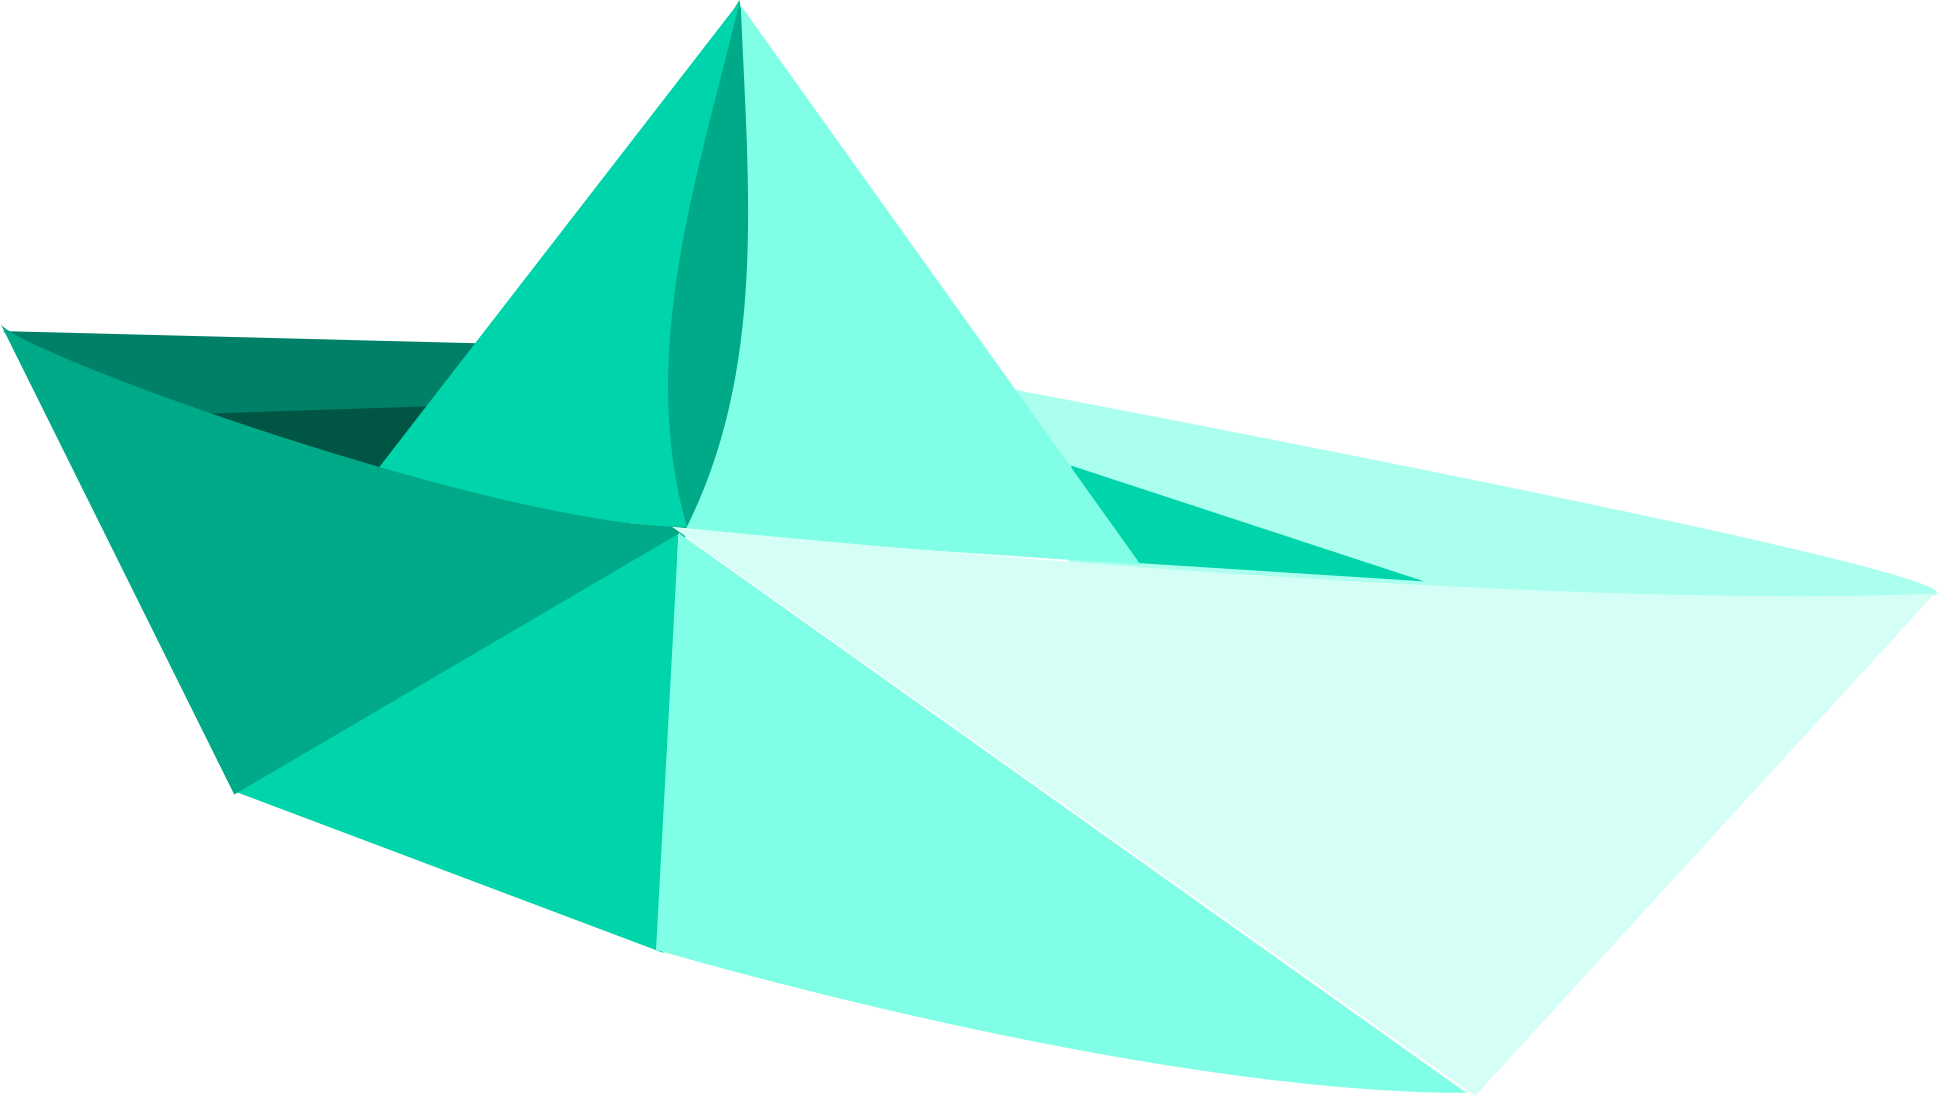
\includegraphics[scale=\myscale,scale=0.4]{figures/badaman-paper-boat}
\end{center}

Cependant tout n'est pas perdu : à partir d'une feuille de papier, un tuto d'origami vous explique comment faire un petit bateau 3D. Si vous avez parfaitement anticipé les pliages et avez colorié votre feuille 2D intelligemment alors une fois formé votre bateau est déjà peint !
Heureusement pour nous pas besoin d'être ingénieux, nous allons considérer que notre objet 3D est déjà découpé en morceaux plat que l'on va décorer un par un.

Ci-dessous une sphère modélisée par un maillage (à gauche), avec un rendu plat (au centre), avec un rendu lisse (à droite).

\begin{center}
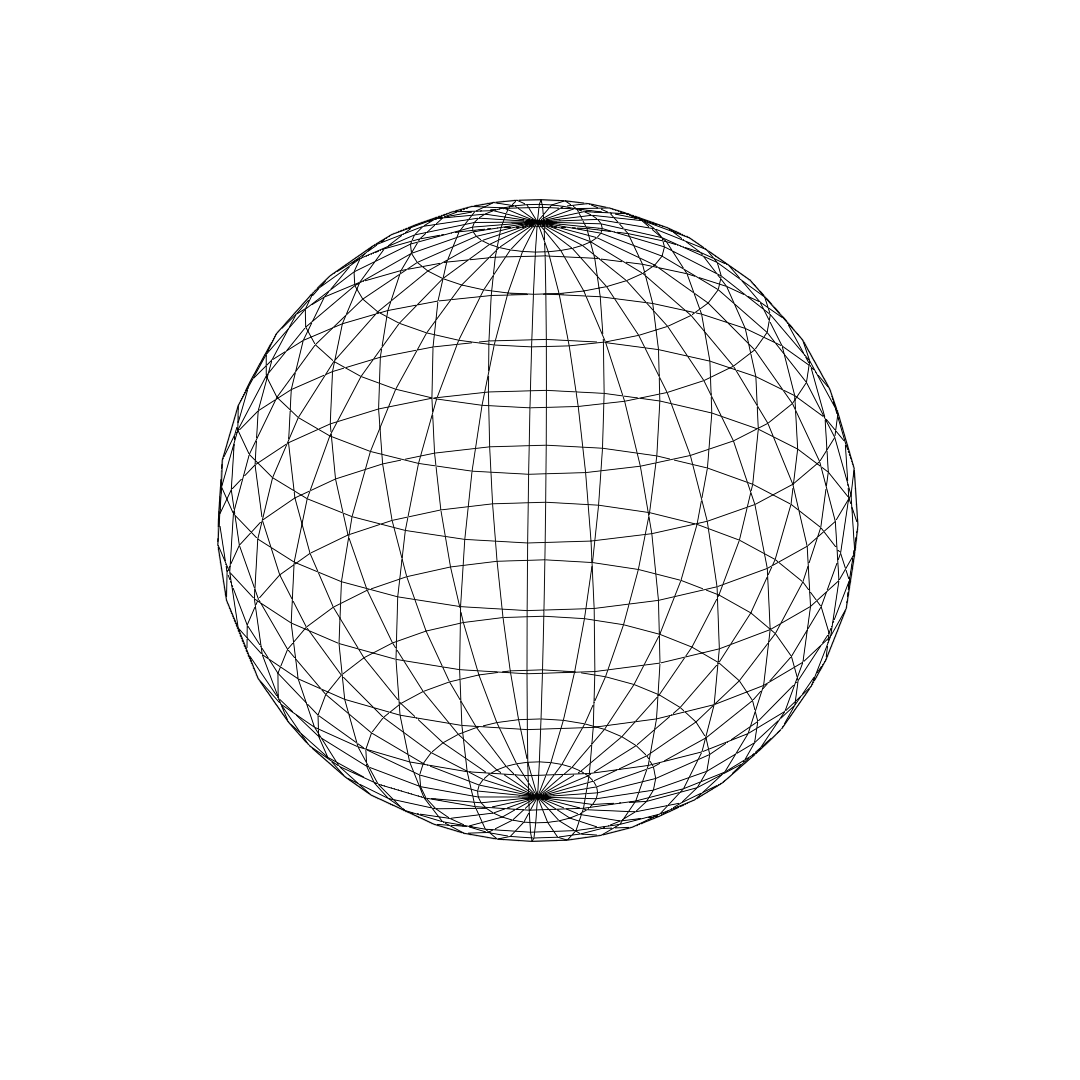
\includegraphics[scale=\myscale,scale=0.15,trim={3cm 7cm 3cm  7cm},clip]{figures/texture-sphere-frame}
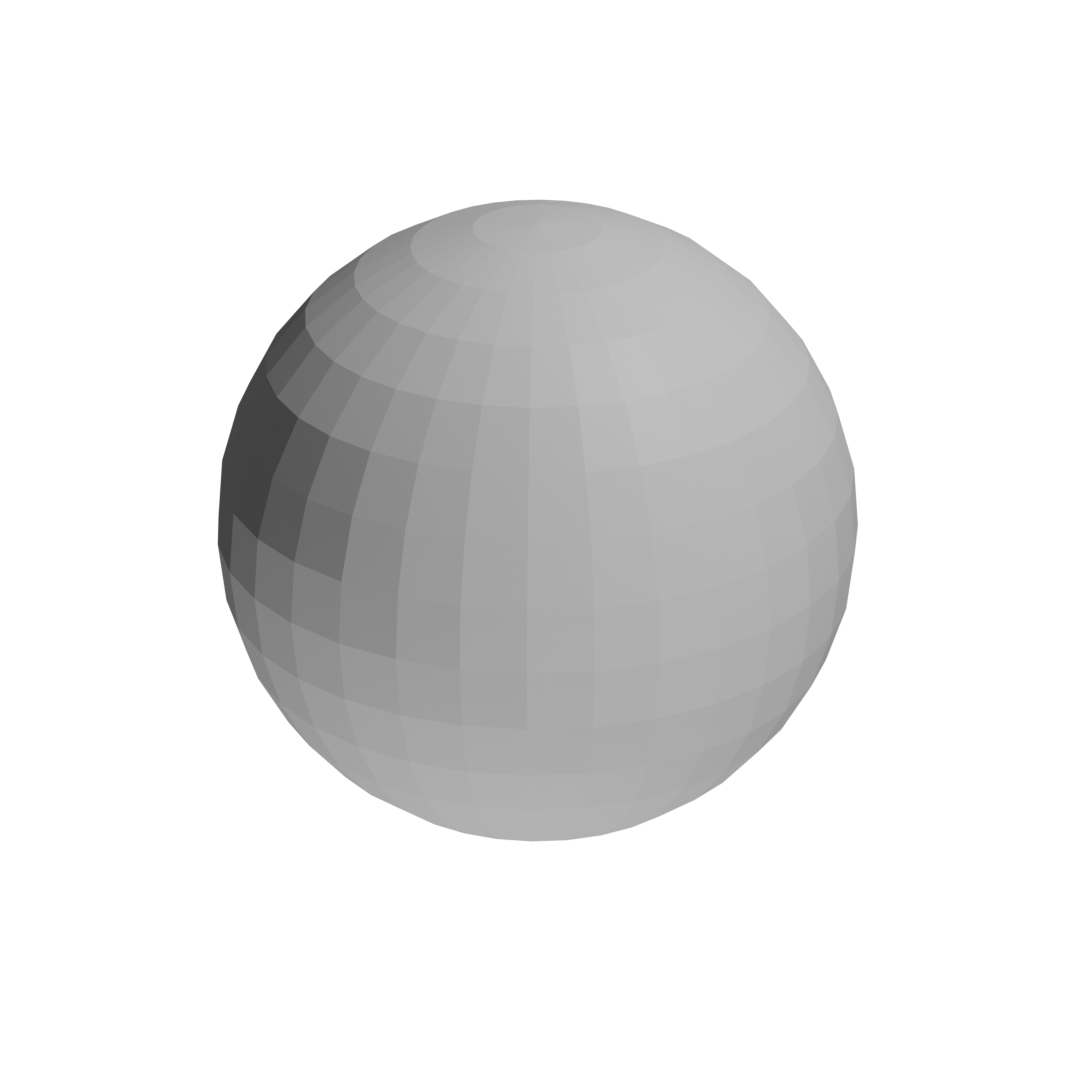
\includegraphics[scale=\myscale,scale=0.15,trim={3cm 7cm 3cm 7cm},clip]{figures/texture-sphere-flat}
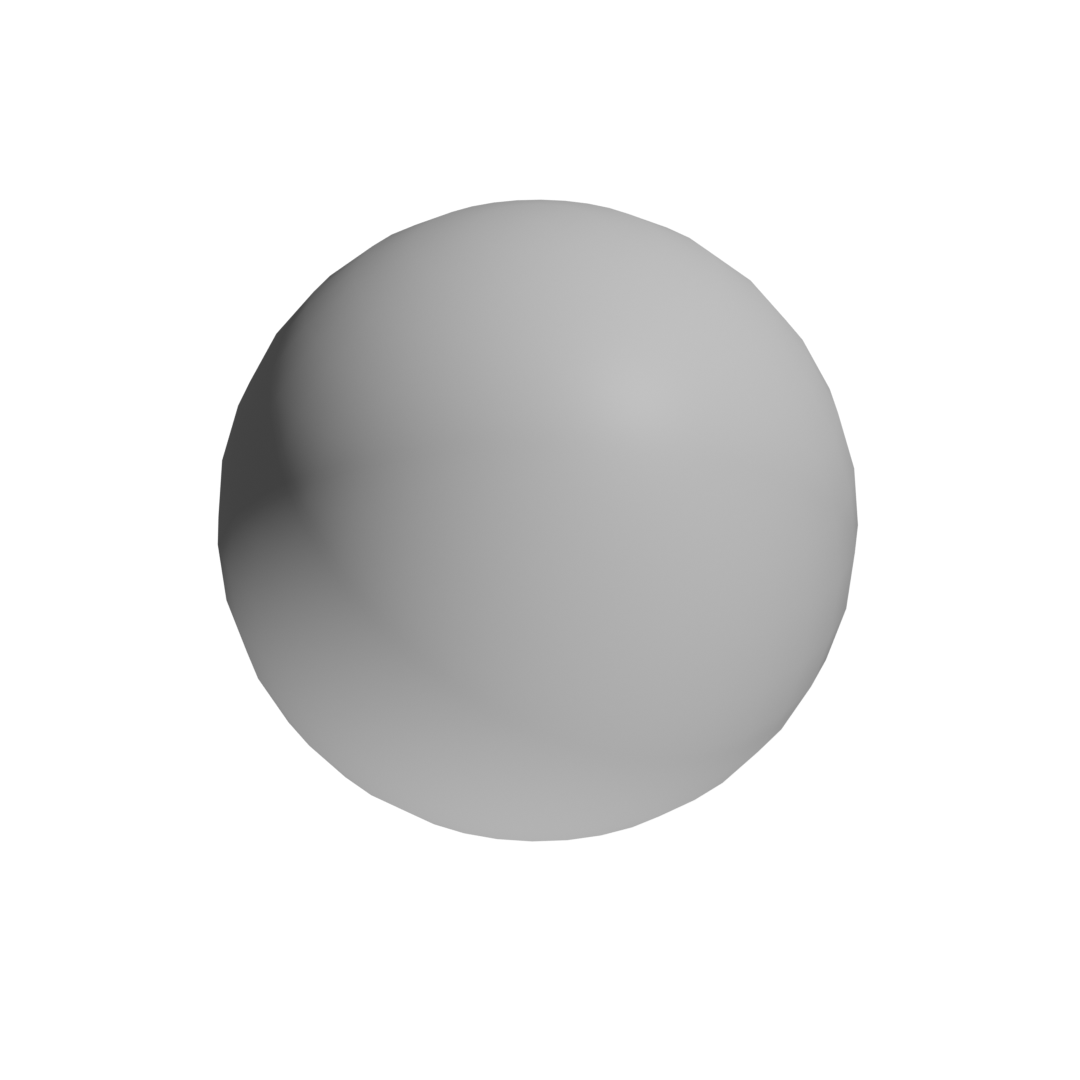
\includegraphics[scale=\myscale,scale=0.15,trim={3cm 7cm 3cm 7cm},clip]{figures/texture-sphere-smooth}
\end{center}

Voici trois images de texture :
\begin{center}
	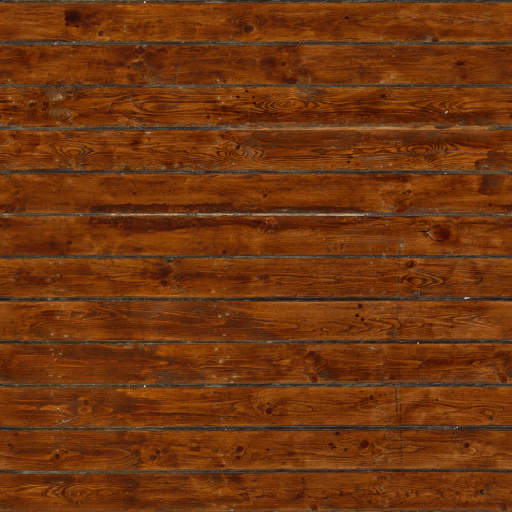
\includegraphics[scale=\myscale,scale=0.61]{figures/carre-texture-wood}
	\qquad\qquad\qquad
	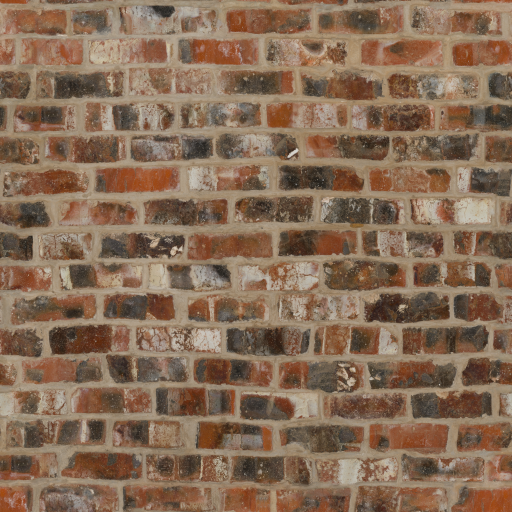
\includegraphics[scale=\myscale,scale=0.61]{figures/carre-texture-brick}
	\qquad\qquad\qquad
	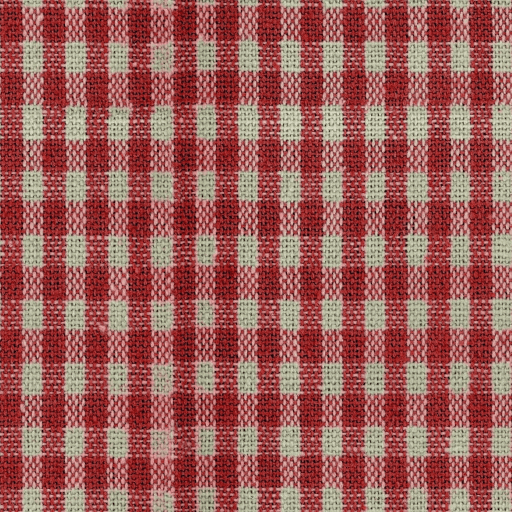
\includegraphics[scale=\myscale,scale=0.15]{figures/carre-texture-coton}
\end{center}

Voici l'application de ces différentes textures :
\begin{center}
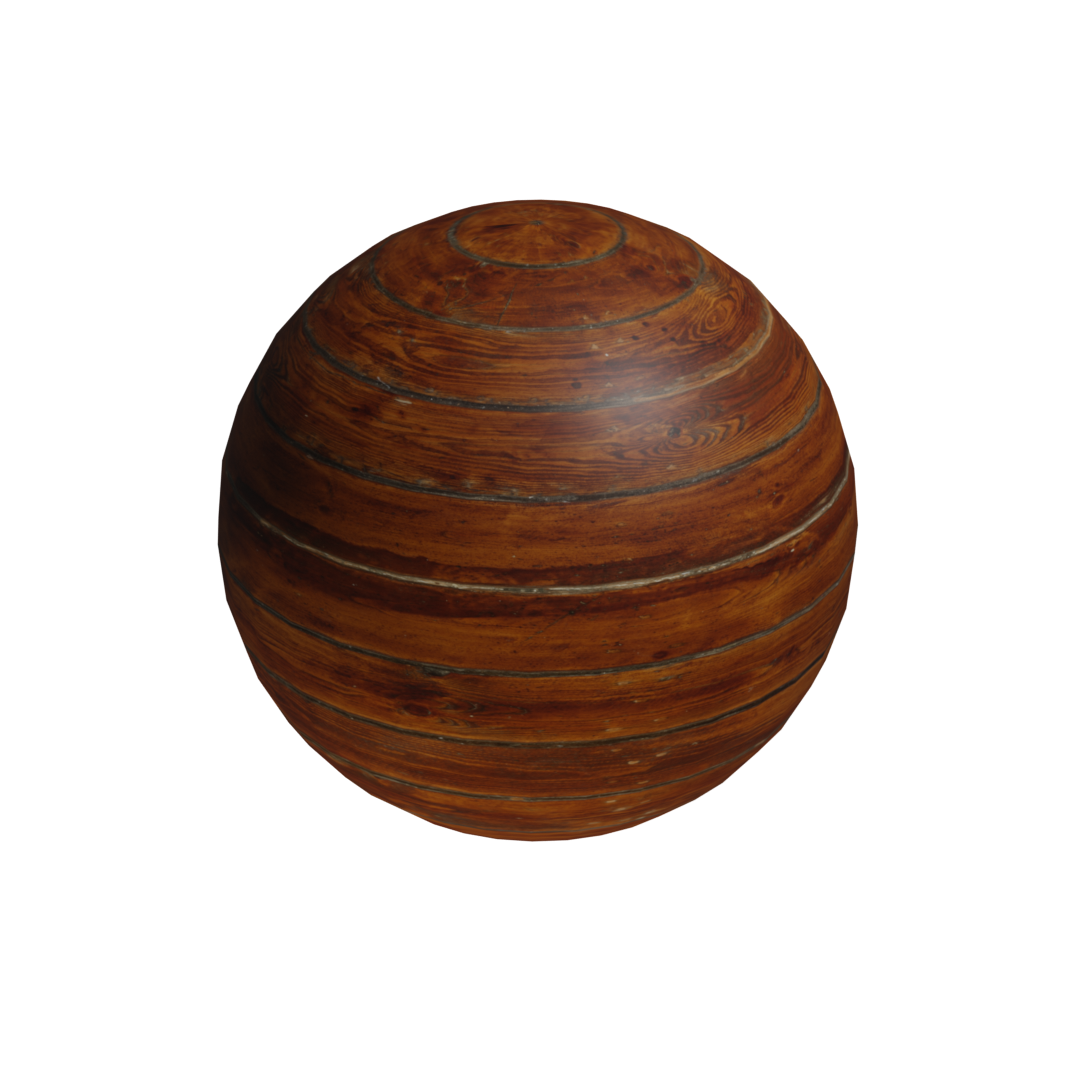
\includegraphics[scale=\myscale,scale=0.15,trim={3cm 7cm 3cm 7cm},clip]{figures/texture-sphere-wood}
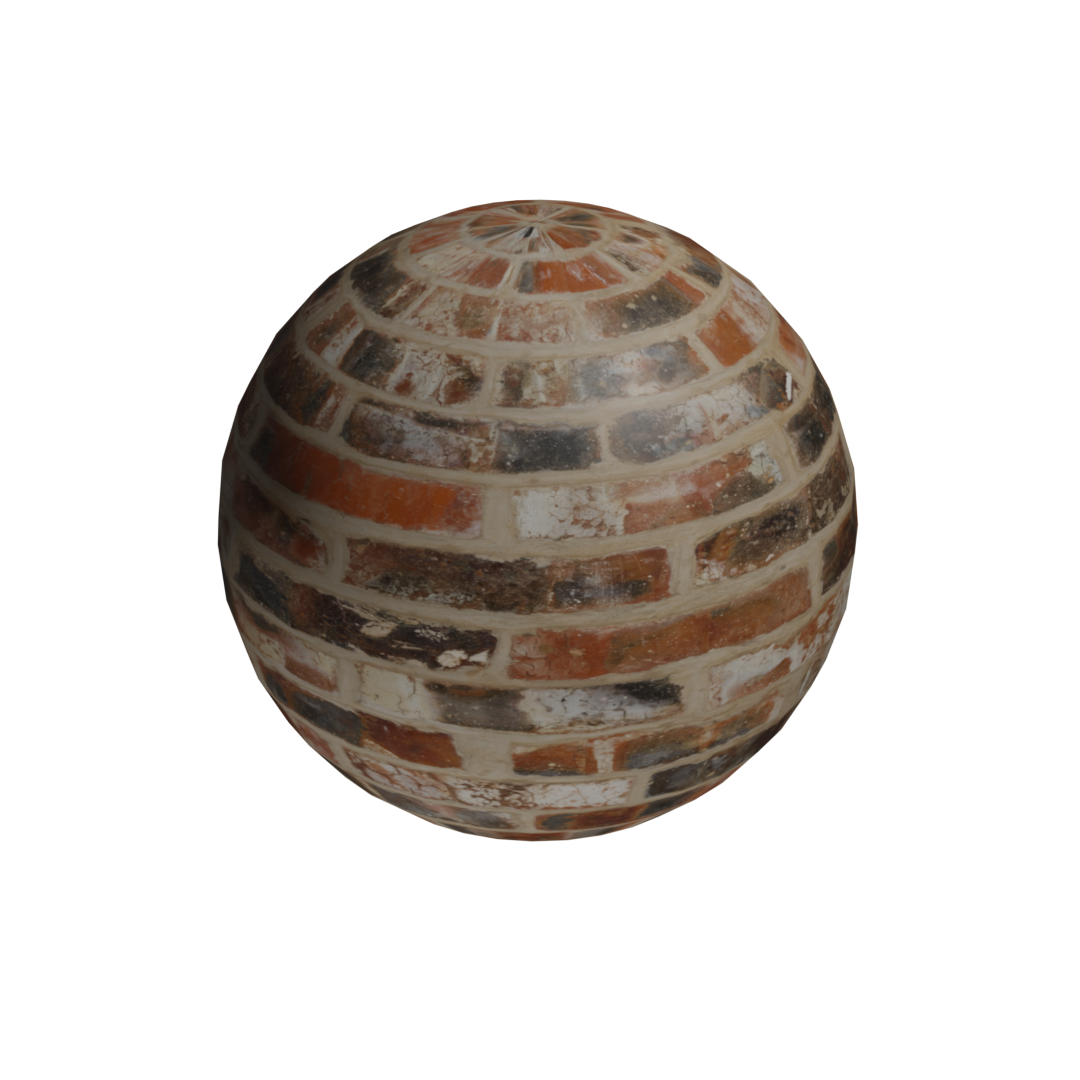
\includegraphics[scale=\myscale,scale=0.15,trim={3cm 7cm 3cm 7cm},clip]{figures/texture-sphere-brick}
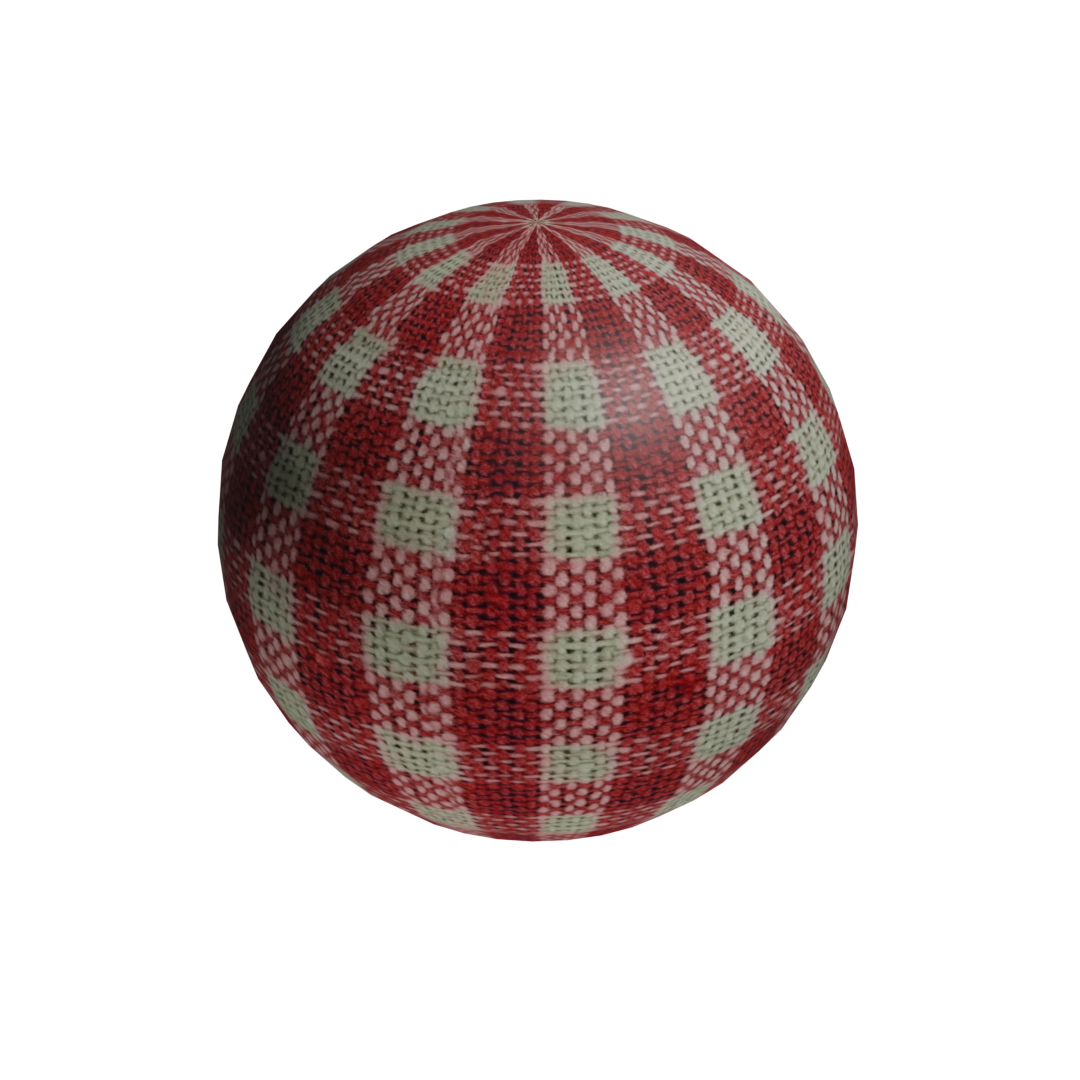
\includegraphics[scale=\myscale,scale=0.15,trim={3cm 7cm 3cm 7cm},clip]{figures/texture-sphere-coton}
\end{center}



Ci-dessous un objet 3D obtenu comme une union de faces (à gauche).
Ce maillage est aplati (à droite) en ce qui s'appelle une \emph{$uv$-map}, c'est sur ce patron 2D que la texture est dessinée avant d'être appliquée sur l'objet 3D.

\begin{center}
%\begin{minipage}{0.25\textwidth}
%	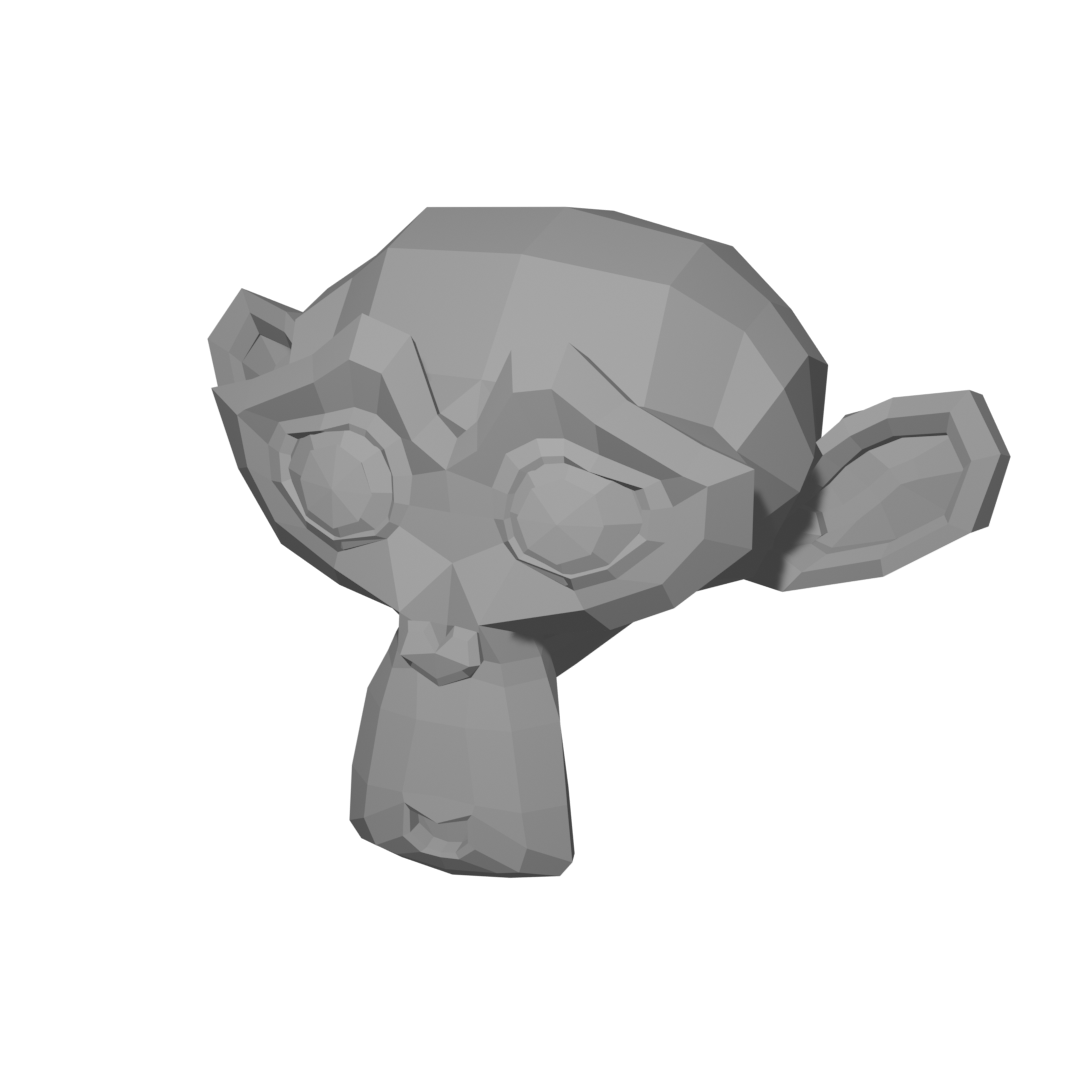
\includegraphics[scale=\myscale,scale=0.14,trim={4cm 3cm 3cm 2.5cm},clip]{figures/uv-map-03-new}
%\end{minipage}
\begin{minipage}{0.5\textwidth}
	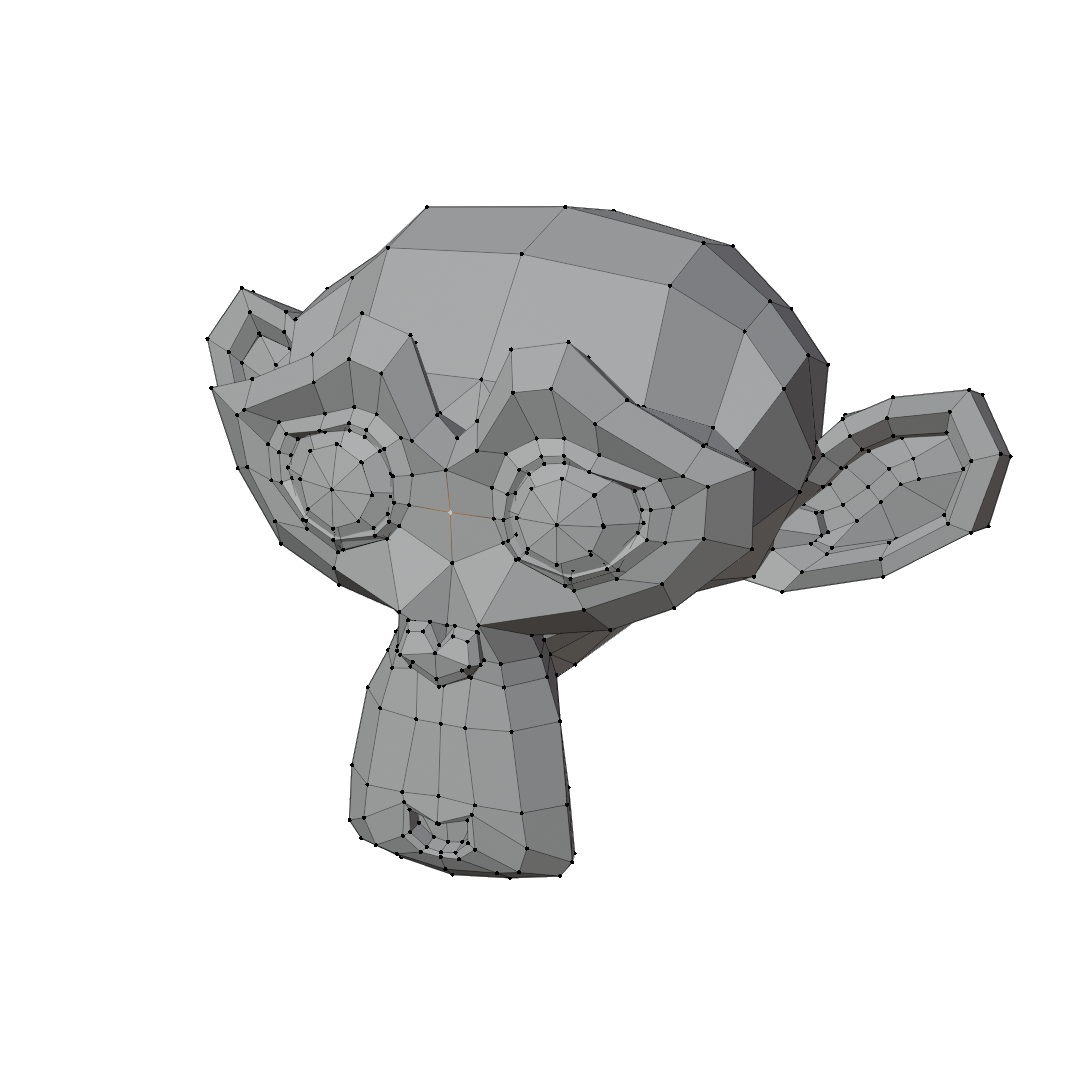
\includegraphics[scale=\myscale,scale=0.20,trim={5cm 3cm 1cm 2.5cm},clip]{figures/uv-map-02-new}    
\end{minipage}\quad
\begin{minipage}{0.45\textwidth}
	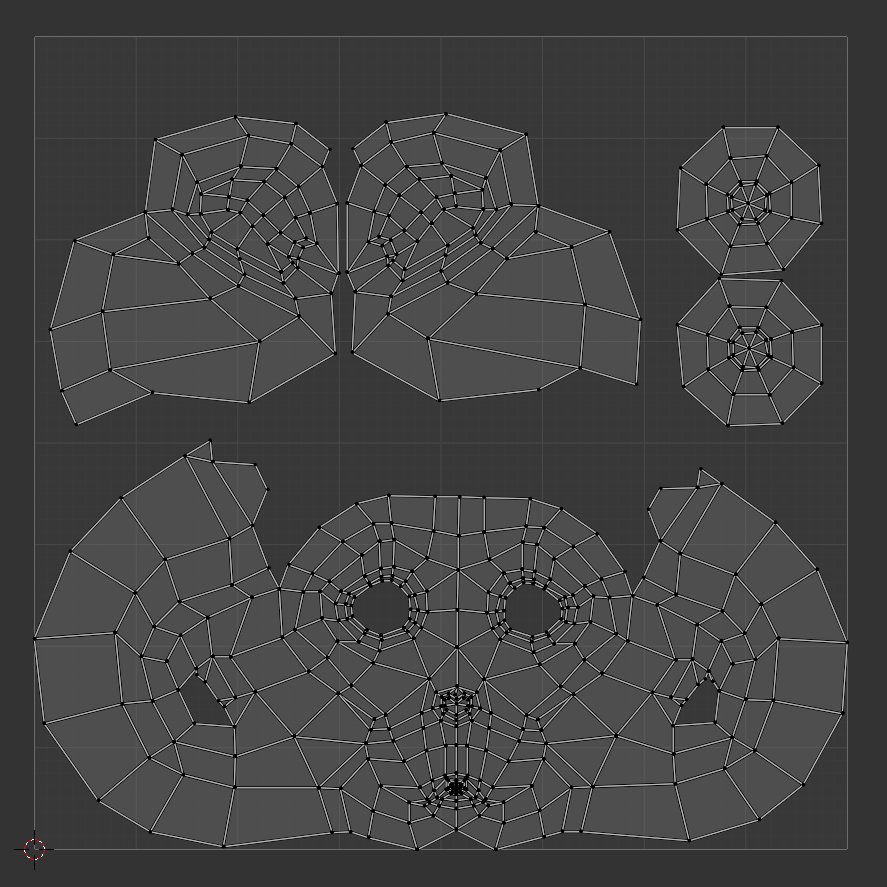
\includegraphics[scale=\myscale,scale=0.19]{figures/uv-map-01}    
\end{minipage}
\end{center}



Quel est l'intérêt d'une texture ?
Tout d'abord cela permet une séparation conceptuelle et pratique entre deux tâches différentes : 
modéliser un objet d'une part et le décorer d'autre part. 
Le texturage lui-même peut se décomposer en plusieurs niveaux : le décor, mais aussi la matière, la granulosité\ldots{}
Ensuite il est plus facile pour un graphiste de créer une jolie texture en 2D que de décorer directement sur l'objet 3D. Enfin, une texture apporte généralement un gain de temps important pour les calculs. Est-il vraiment utile de modéliser chaque brique d'un mur ou chaque carré de pelouse surtout s'il s'agit d'un décor assez lointain ?

%--------------------------------------------------------------------
\subsection{Texture (dimension 1)}


L'idée pour appliquer une texture est simple : on part d'une image et on la colle sur un objet. Voyons ce que pourrait être une définition mathématique.
Nous commençons à chaque fois les explications en une seule dimension. Même si une texture en dimension $1$ a peu d'utilité, les concepts sont les mêmes que pour la dimension $2$ mais les équations sont plus simples.

Une \defi{texture} (en dimension $1$) est une fonction :
$$
	\begin{array}{rcl}
	\mathcal{C} : [0,1] & \longrightarrow & E \\
	 u & \longmapsto & \mathcal{C}(u)
	 \end{array}
$$
	 
Explications : on part de l'intervalle de référence $[0,1]$, à chaque point de cet intervalle on associe une valeur appartenant à un ensemble $E$. 
Le cas le plus fréquent est d'associer une couleur $\mathcal{C}(u)$ à chaque point $u \in [0,1]$, par exemple sous la forme d'une valeur $\mathcal{C}(u) = (r,g,b) \in [0,1]^3$. Autrement dit, il s'agit de colorier chaque pixel de l'intervalle fixe $[0,1]$.

\myfigure{1}{
	\tikzinput{fig-texture-01}		
}



Considérons maintenant un objet $O$ et une de ses faces $F$. Si l'objet est dans le plan, une face $F$ est un intervalle $[A,B]$ du plan.
La \defi{fonction de plaquage} est une application bijective $\Phi$:
$$  \begin{array}{rcl}
	\Phi : [0,1] & \longrightarrow & F \\
	u & \longmapsto & \Phi(u)
\end{array}
$$ 
	
Nous notons $\Psi = \Phi^{-1}$ sa bijection réciproque, qui nous sera utile : 
$$  \begin{array}{rcl}
	\Psi : F & \longrightarrow & [0,1] \\
	P & \longmapsto & \Psi(P)
\end{array}
$$

\defi{Appliquer une texture} c'est l'action de $\mathcal{C} \circ \Psi$, c'est-à-dire associer à chaque $P$ de la face $F$ une couleur par la fonction :
$$\mathcal{C}\big(\Psi(P)\big)$$

Autrement dit :
\begin{itemize}
	\item pour déterminer la couleur de $P$, on calcule à quel paramètre $u\in[0,1]$ il correspond : $u = \Psi(P)$. 
	La couleur de $P$ est celle de $u$ : $\mathcal{C}(u)$. 
	Cette façon de faire est le \emph{texturage inverse} : on part du pixel de l'objet à colorier et on cherche sa couleur par l'application inverse $\Psi$.
	
	\item une autre façon de procéder est le \emph{texturage direct} : pour chaque $u\in [0,1]$ on calcule $P = \Phi(u)$ et on le colorie par la couleur $\mathcal{C}(u)$.
\end{itemize}	

Quelques remarques. Le texturage ne se limite pas à associer une couleur, nous verrons des exemples d'autres situations un peu plus tard.
On pourrait aussi considérer une face $F$ qui ne soit pas un segment, un arc de cercle par exemple.

%--------------------------------------------------------------------
\subsection{Texture (dimension 2)}


Une \defi{texture} (en dimension $2$) est une fonction :
$$\begin{array}{rcl}
	\mathcal{C} : [0,1]^2 & \longrightarrow & E \\
	(u,v) & \longmapsto & \mathcal{C}(u,v)
\end{array}
$$
C'est une fonction qui à chaque point $(u,v)$ d'un carré de référence associe une valeur. Autrement dit chaque pixel du carré est colorié.
Pour un objet $O$ (de l'espace) et une de ses faces $F$, la \defi{fonction de plaquage} est une application bijective $\Phi$:
$$  \begin{array}{rcl}
	\Phi : [0,1]^2 & \longrightarrow & F \\
	(u,v) & \longmapsto & \Phi(u,v)
\end{array}
$$ 
Sa réciproque étant :
$$  \begin{array}{rcl}
	\Psi : F & \longrightarrow & [0,1]^2 \\
	P & \longmapsto & \Psi(P)
\end{array}
$$	

\defi{Appliquer la texture}, c'est pour chaque $P \in F$ lui associer la couleur $\mathcal{C}\big(\Psi(P)\big)$.

\myfigure{0.9}{
	\tikzinput{fig-texture-02}		
}


%--------------------------------------------------------------------
\subsection{Texture (dimension 1) : suite}

Revenons à nos textures en dimension $1$.

\textbf{Interpolation linéaire de $[0,1]$ dans $[a,b]$.}
Tout d'abord, le choix de l'intervalle $[0,1]$ comme ensemble de départ des fonctions $\mathcal{C}$ et $\Phi$ est un peu arbitraire.
On passe facilement de l'intervalle $[0,1] \subset \Rr$ à n'importe quel intervalle $[a,b] \subset \Rr$ (avec $a \neq b$), pour cela il suffit de considérer la bijection :
$$  \begin{array}{rcl}
	\phi : [0,1] & \longrightarrow & [a,b] \\
	u & \longmapsto & (1-u)a + u b
\end{array}
$$ 
C'est l'exemple basique d'interpolation linéaire (\emph{lerp}) : $0$ s'envoie sur $a$, $1$ sur $b$, $\frac12$ sur $\frac{a+b}{2}$\ldots




\textbf{Interpolation non linéaire.}
Si $a=0$ et $b=1$ alors la fonction $\phi$ précédente est tout simplement l'identité $\phi(x)=x$.
Mais il existe beaucoup d'autres fonctions $f : [0,1] \to [0,1]$ qui sont bijectives, 
par exemple toute fonction $f$ continue, strictement croissante avec $f(0)=0$ et $f(1)=1$.
Une analogie c'est parcourir \SI{10}{\kilo\meter} en \SI{1}{\hour}, on peut le faire à vitesse constante, ou bien rapide puis lent, ou l'inverse\ldots{}
De telles interpolations non linéaires peuvent être utiles. 
\myfigure{0.8}{
	\tikzinput{fig-texture-03}		
}

Dans la suite on se limitera aux interpolations linéaires.

\textbf{Interpolation linéaire de $[0,1]$ dans $[A,B]$.}

Pour $A,B$ deux points du plan (ou de l'espace), la fonction de plaquage $\Phi : [0,1] \to [A,B]$ naturelle est celle de l'interpolation linéaire :
$$\Phi(u) = (1-u) A + u B.$$


\myfigure{0.8}{
	\tikzinput{fig-texture-04}		
}

Autrement dit, $P = (1-u) A  + u B$, ou encore en termes de vecteurs $\vec{AP} = u \vec{AB}$.
Si on note $A(x_A,y_A)$ et $B(x_B,y_B)$ alors : 
$$
P = \begin{pmatrix} x \\ y \end{pmatrix}
= (1-u) \begin{pmatrix} x_A \\ y_A \end{pmatrix} + u \begin{pmatrix} x_B \\ y_B \end{pmatrix}
= \begin{pmatrix} (1-u)x_A + u x_B \\ (1-u)y_A + u y_B \end{pmatrix}
= \begin{pmatrix} x_A + u (x_B-x_A) \\ y_A + u (y_B-y_A) \end{pmatrix}
.$$
Il s'agit en fait de l'interpolation linéaire sur chacune des coordonnées.
Les formules sont similaires pour $A(x_A,y_A,z_A)$ et $B(x_B,y_B,z_B)$ des points de l'espace.


%--------------------------------------------------------------------
\subsection{Équations directes et inverses}

Interprétons les calculs précédents en termes de matrices. Les coordonnées $(x,y)$ de $P = \Phi(u)$ se calculent par :
$$\begin{pmatrix} x \\ y \end{pmatrix} = T \begin{pmatrix} u \\ 1 \end{pmatrix}$$
avec 
$$T = \begin{pmatrix}
x_B-x_A & x_A \\
y_B-y_A & y_A 	
\end{pmatrix}.$$

La preuve est juste une variante des écritures précédentes :
$$\left\{
\begin{array}{rcl}
	x &=& u(x_B - x_A) + x_A \\
	y &=& u(y_B - y_A) + y_A \\	
\end{array}
\right..$$
Ces formules définissent $\Phi : [0,1] \to [A,B]$.

Réciproquement on pourrait calculer $u$ à l'aide de 
$$\begin{pmatrix} u \\ 1 \end{pmatrix} = T^{-1} \begin{pmatrix} x \\ y \end{pmatrix}$$
Mais un calcul direct donne ici :
$$u = \frac{x-x_A}{x_B-x_A} = \frac{y-y_A}{y_B-y_A}.$$
Cette formule définit $\Psi : [A,B] \to [0,1]$.


%--------------------------------------------------------------------
\subsection{Modifications selon la normale}

Les textures sont utiles bien au-delà de l'ajout d'une couleur.
Les textures permettent : des effets de relief, de modifier la granulosité, modifier la matière, modifier l'effet de l'éclairage, d'ajouter de la transparence et de modifier localement la forme de l'objet.

Nous allons nous intéresser à la modification locale de la forme de l'objet qui peut être réelle ou simulée. Cela permet de donner du relief, comme par exemple la peau d'une orange.
Nous allons voir trois méthodes de la plus simple à celle qui demande le plus de calculs.

\textbf{\emph{Bump map.}}\index{texture!bump map@\emph{bump map}}
Il s'agit de modifier la hauteur apparente de la surface en simulant un léger déplacement selon la direction normale.
Mathématiquement, en dimension $1$,  cette texture est une fonction $\mathcal{C} : [0,1] \to \Rr$ qui à un paramètre $u$ associe une hauteur $\mathcal{C}(u)$ de déplacement.

\myfigure{0.8}{
	\tikzinput{fig-texture-05}		
}


En dimension $2$ ce serait $\mathcal{C} : [0,1]^2 \to \Rr$ et informatiquement, cette texture est stockée par une \emph{heigthmap}, c'est-à-dire une image en niveaux de gris qui représentent des hauteurs.
Ci-dessous à gauche une image en niveaux de gris, les pixels blancs correspondant aux points les plus hauts et les pixels noirs aux points les plus bas. Sur la figure de droite le rendu 3D correspondant (ici un carré de côté \SI{30}{\kilo\meter} autour de la source de la Loire), un facteur d'échelle permet d'obtenir un terrain plus ou moins plat (ici le rendu 3D est réel et correspond à la \emph{displacement map} plus bas).
\begin{center}
	\begin{minipage}{0.45\textwidth}
		
\includegraphics[scale=\myscale,angle=-90,scale=0.15]{figures/heightmap_loire_bis}
	\end{minipage}
	\begin{minipage}{0.5\textwidth}
		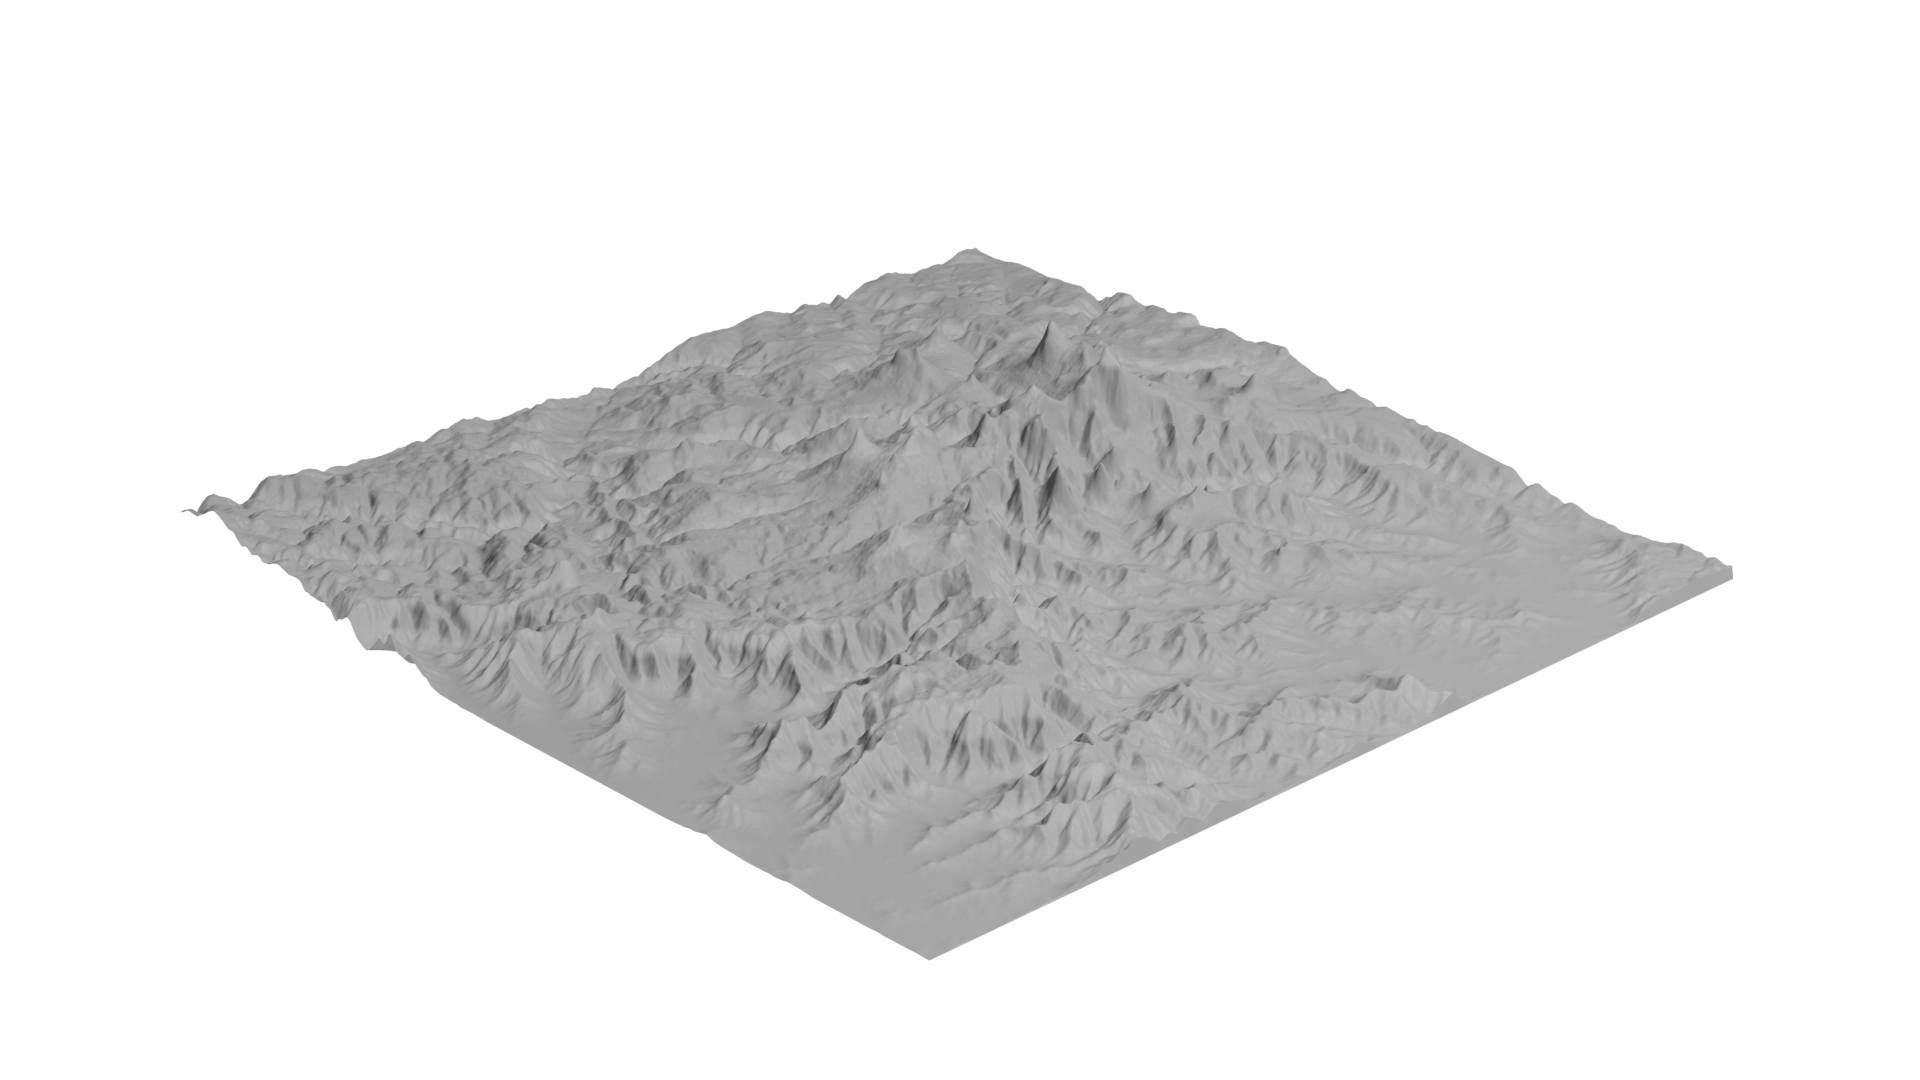
\includegraphics[scale=\myscale,scale=0.17,trim={8cm 0 5cm 0}, clip]{figures/3D-loire}    
	\end{minipage}
\end{center}


Revenons au cas d'une texture de dimension $1$. Pour un point $P$ de la face $[A,B]$ de paramètre $u=\Psi(P)$, au lieu d'afficher le point $P$ on aimerait afficher le point $Q = P + \mathcal{C}(u) \vec{n_P}$.



\myfigure{0.8}{
	\tikzinput{fig-texture-06}		
}


Cette modification est \og{}simulée\fg{} car on ne va pas modifier la géométrie réelle de l'objet, on ne retient que la modification de la normale, autrement dit le changement d'éclairage de l'objet.
Disons, pour simplifier, que pour dessiner et éclairer un point d'un objet on a juste besoin de connaître la position de ce point $P$ et le vecteur normal à l'objet en ce point $\vec{n_P}$ (voir le chapitre \og{}Lumière\fg{}).
Ici on va bien tracer le point en $P$ mais avec le vecteur normal $\vec{n_{Q}}$ correspondant au point $Q$. 
Le calcul de  $\vec{n_{Q}}$ se fait à l'aide de $\vec{n_P}$ et de la fonction $u \mapsto \mathcal{C}(u)$.
Ces calculs sont simples et permettent de simuler efficacement des effets réalistes. 
Cependant la géométrie de l'objet n'a pas changé : un rayon lancé sur notre objet  intersecte toujours l'objet sur la face initiale et pas sur la face simulée.
Par exemple l'ombre de l'objet ne change pas.



\medskip

\textbf{\emph{Normal map.}}\index{texture!normal map@\emph{normal map}}
Il s'agit d'une variante de la modification précédente, mais cette fois la texture décrit le nouveau vecteur normal à considérer.
Mathématiquement, en dimension $1$,  cette texture est une fonction $\mathcal{C} : [0,1] \to \Rr^3$ qui à un paramètre $u$ associe une modification du vecteur normal.
En dimension $2$ ce serait $\mathcal{C} : [0,1]^2 \to \Rr^3$ et informatiquement, cette texture est stockée par une image couleur \emph{rgb}, chaque niveau de rouge/vert/bleu désignant une des coordonnées $(x,y,z)$. 

Il y a donc beaucoup plus de liberté que pour la \emph{bump map}
et l'effet peut être plus réaliste. Il permet même de réduire drastiquement la taille d'un maillage ou d'une triangulation tout en gardant un rendu 3D de qualité.
Comme précédemment la géométrie réelle de l'objet n'est pas changée, on remplace le vecteur normal $\vec{n_P}$ en $P$ par un nouveau vecteur $\vec{n'_P}$ calculé à partir de 
$\vec{n_P}$ et de $\mathcal{C}(u)$. C'est ce nouveau vecteur $\vec{n'_P}$ qui est utilisé en tant que vecteur normal lors de l'éclairage.


\begin{center}
	\begin{minipage}{0.32\textwidth}	
		\center
		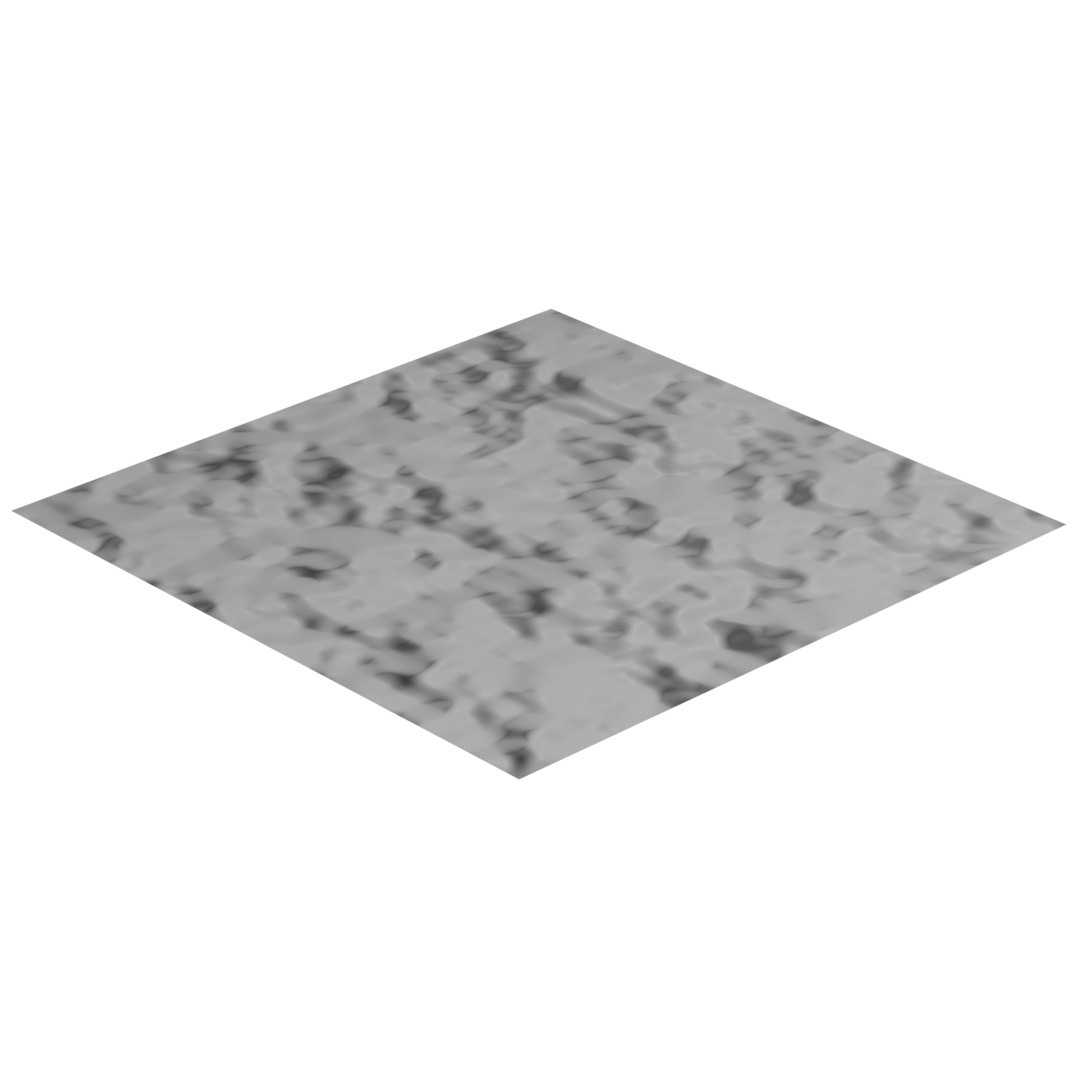
\includegraphics[scale=\myscale,scale=0.13,trim={0 8cm 0 8cm},clip]{figures/texture-plan-bump}
		
		\emph{Bump/Normal}
	\end{minipage}	
	\begin{minipage}{0.32\textwidth}
		\center
		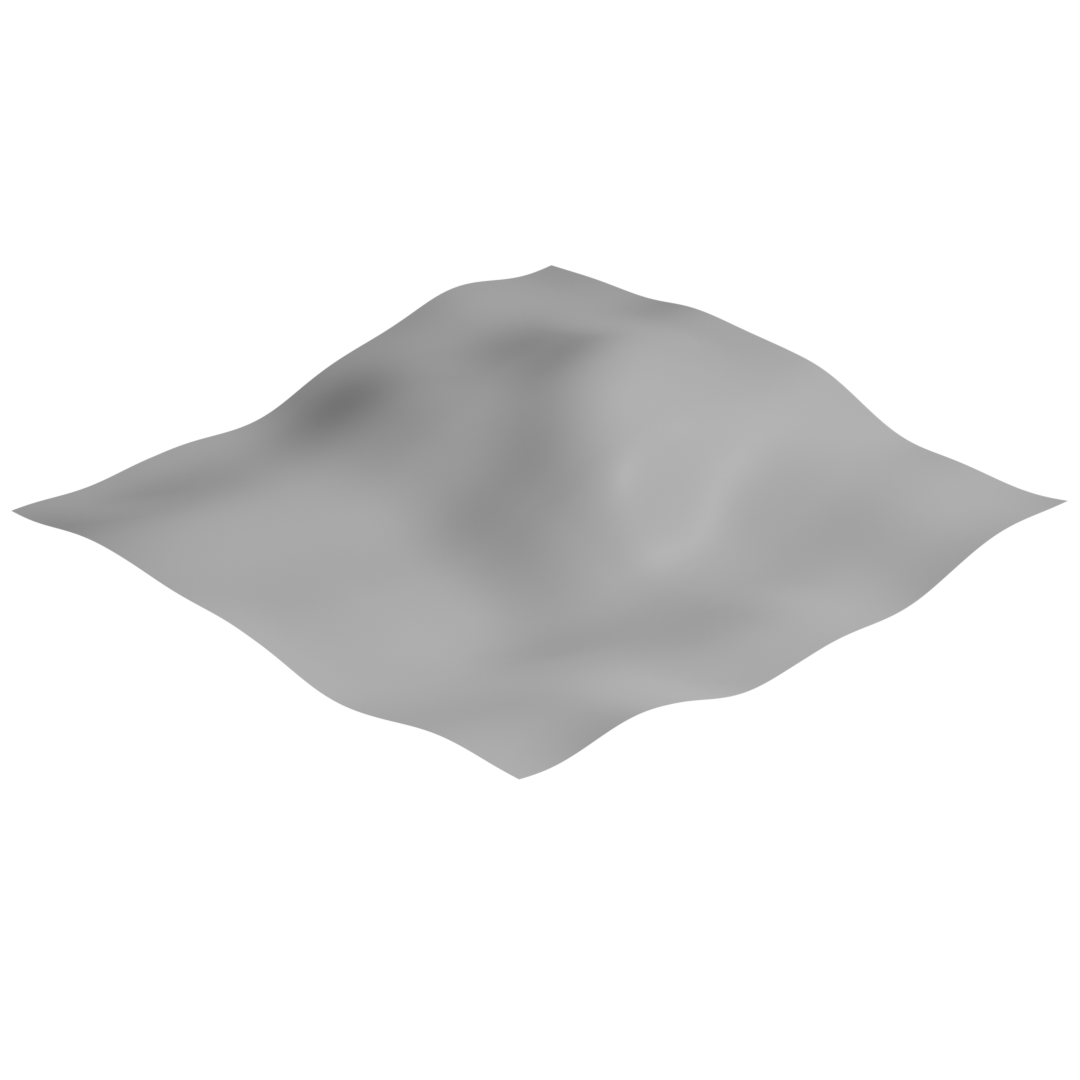
\includegraphics[scale=\myscale,scale=0.13,trim={0 8cm 0 8cm},clip]{figures/texture-plan-bump-dis1}
		
		
		\emph{Displacement} (facteur 1)
	\end{minipage}	
	\begin{minipage}{0.32\textwidth}
		\center
		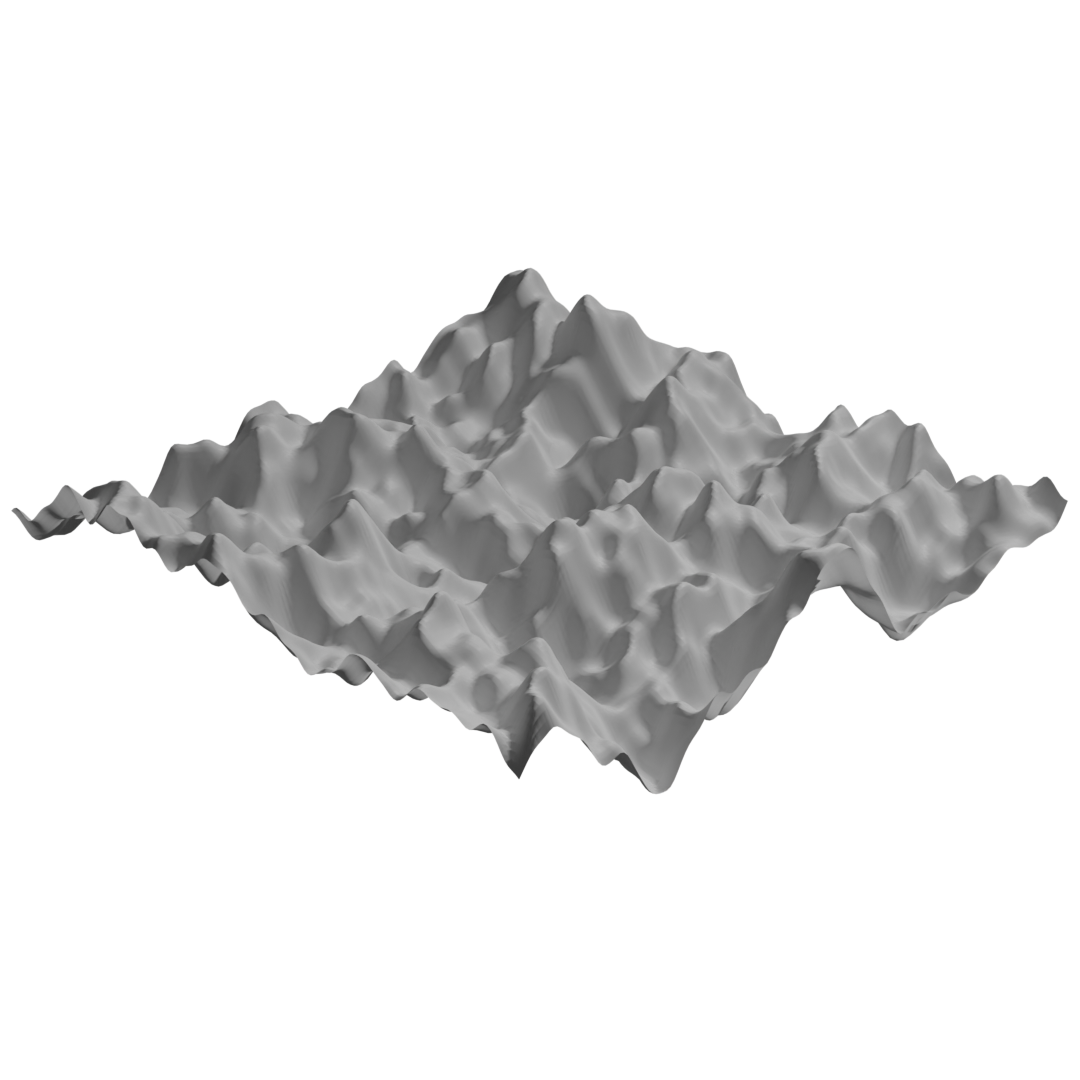
\includegraphics[scale=\myscale,scale=0.13,trim={0 8cm 0 8cm},clip]{figures/texture-plan-bump-dis2}
		
		
		\emph{Displacement} (facteur 2)	
	\end{minipage}	
\end{center}

\medskip

\textbf{\emph{Displacement map.}}\index{texture!displacement map@\emph{displacement map}}
Cette modification est très similaire à la modification précédente, sauf que cette fois on déplace effectivement le point.
La texture est de nouveau une application $\mathcal{C} : [0,1] \to \Rr^3$ (dimension $1$) ou $\mathcal{C} : [0,1]^2 \to \Rr^3$ (dimension $2$).
Le point $P$ est remplacé par le point $Q = P + \vec{n'_P}$.
Ainsi tous les calculs pour les éclairages, les ombres, les lancers de rayons\ldots{} se font à l'aide de cette nouvelle surface. Comme la surface déplacée est plus compliquée que la face originale les calculs sont plus longs.

Voici la déformation d'une sphère obtenue à partir d'un déplacement. Ici la texture est un bruit aléatoire. Un facteur d'échelle permet d'accentuer plus ou moins la déformation. 
\begin{center}	
	\begin{minipage}{0.32\textwidth}
		\center
		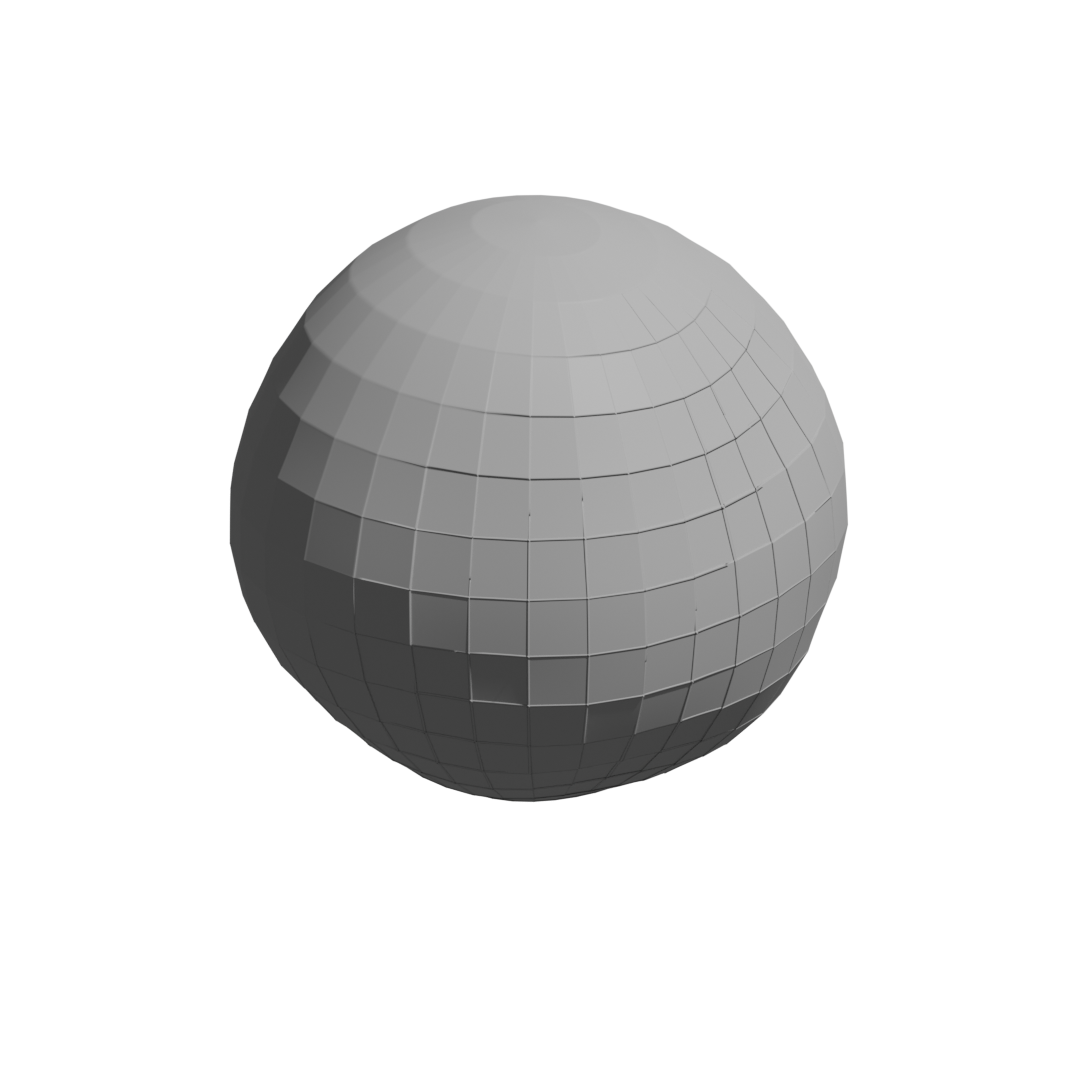
\includegraphics[scale=\myscale,scale=0.13,trim={0 8cm 0 6cm},clip]{figures/texture-sphere-dis1}
		
		\emph{Displacement} (facteur 1)
	\end{minipage}	
	\qquad\qquad
	\begin{minipage}{0.32\textwidth}
		\center
		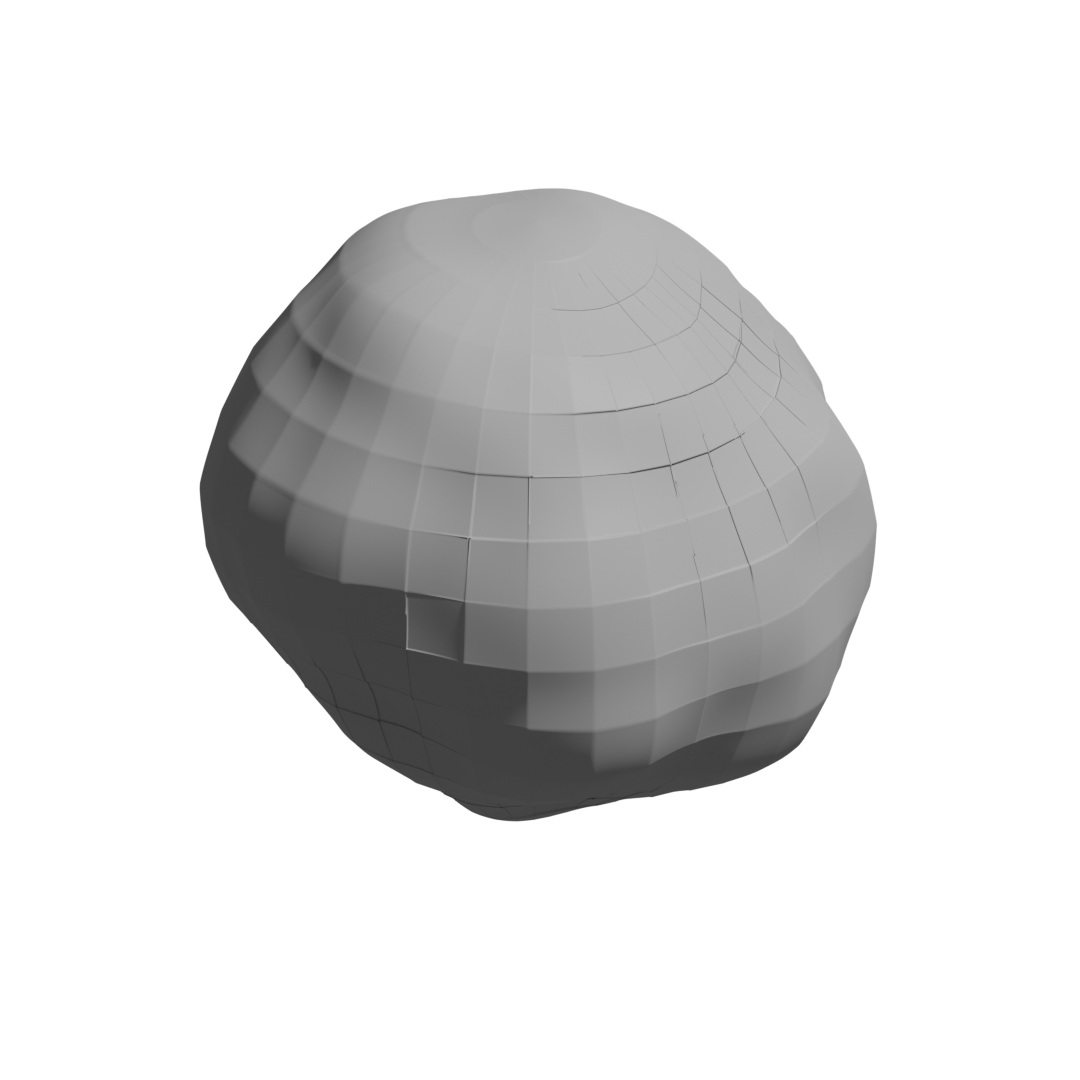
\includegraphics[scale=\myscale,scale=0.13,trim={0 8cm 0 6cm},clip]{figures/texture-sphere-dis2}
		
		\emph{Displacement} (facteur 2)	
	\end{minipage}	
\end{center}

Ci-dessous un résumé des trois modifications : 
à gauche la \emph{bump map}, la surface réelle de l'objet n'est pas modifiée mais le vecteur normal peut être changé avec un degré de liberté ; 
au centre la \emph{normal map}, la surface réelle de l'objet n'est pas non plus modifiée mais le vecteur normal peut être changé avec trois degrés de liberté ;
à droite la \emph{displacement map} la surface réelle de l'objet est modifiée.
\myfigure{1}{
	\tikzinput{fig-texture-07}		
}

\begin{center}
\begin{minipage}{0.32\textwidth}	
	\center
	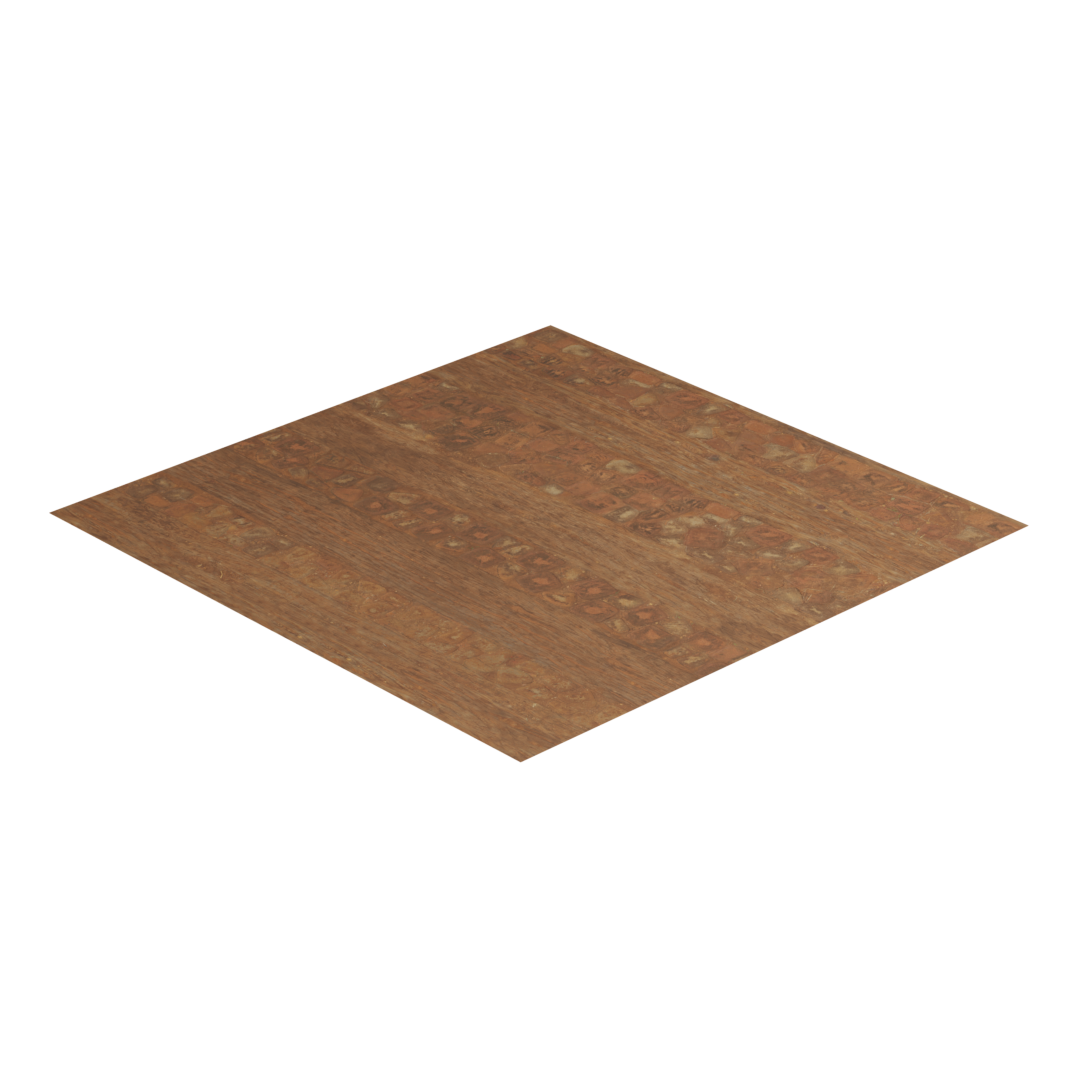
\includegraphics[scale=\myscale,scale=0.15,trim={0 8cm 0 8cm},clip]{figures/texture-wood-flat}
	
	Plat
\end{minipage}	
\begin{minipage}{0.32\textwidth}
	\center
	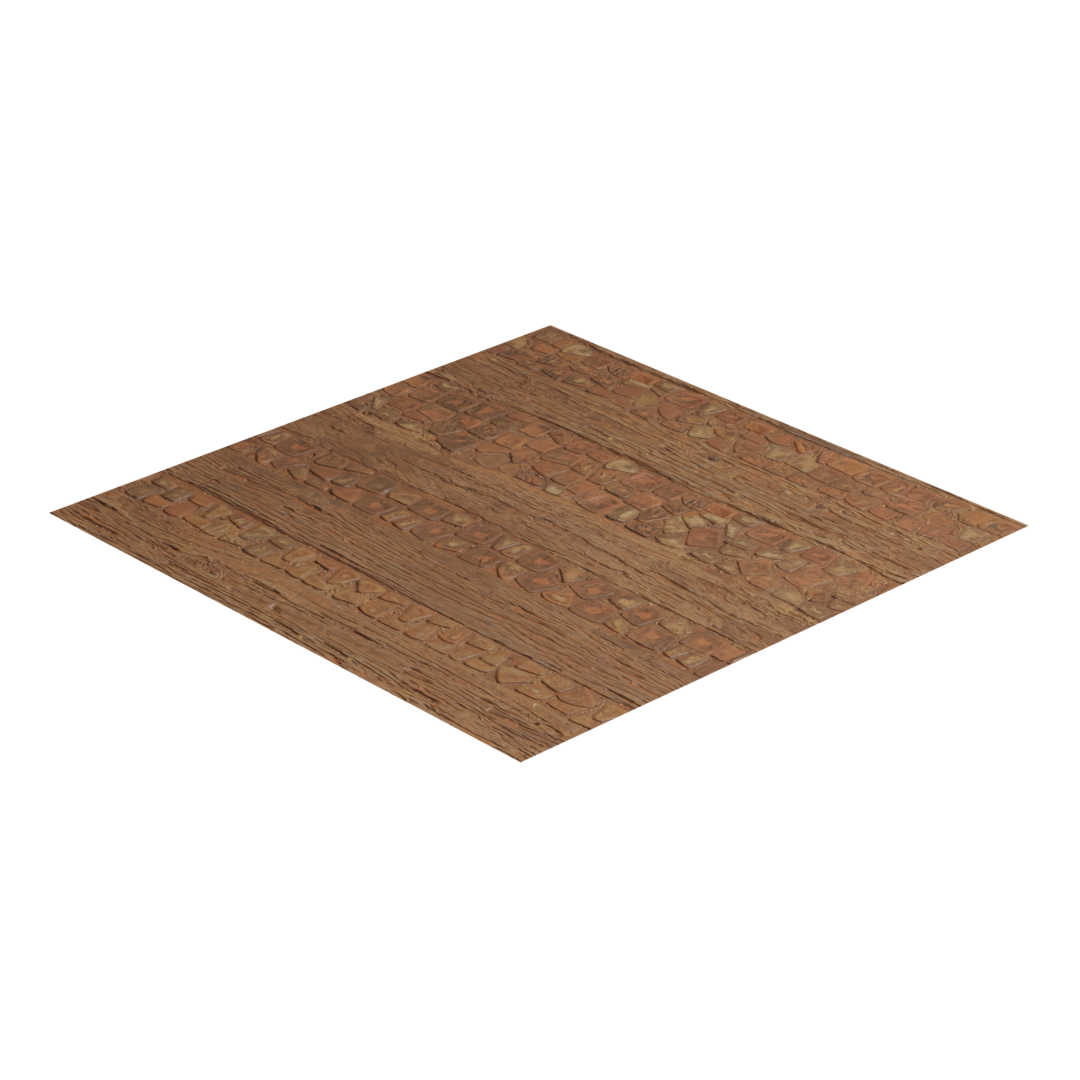
\includegraphics[scale=\myscale,scale=0.15,trim={0 8cm 0 8cm},clip]{figures/texture-wood-bump}
	
		
	\emph{Bump/Normal}
\end{minipage}	
\begin{minipage}{0.32\textwidth}
	\center
	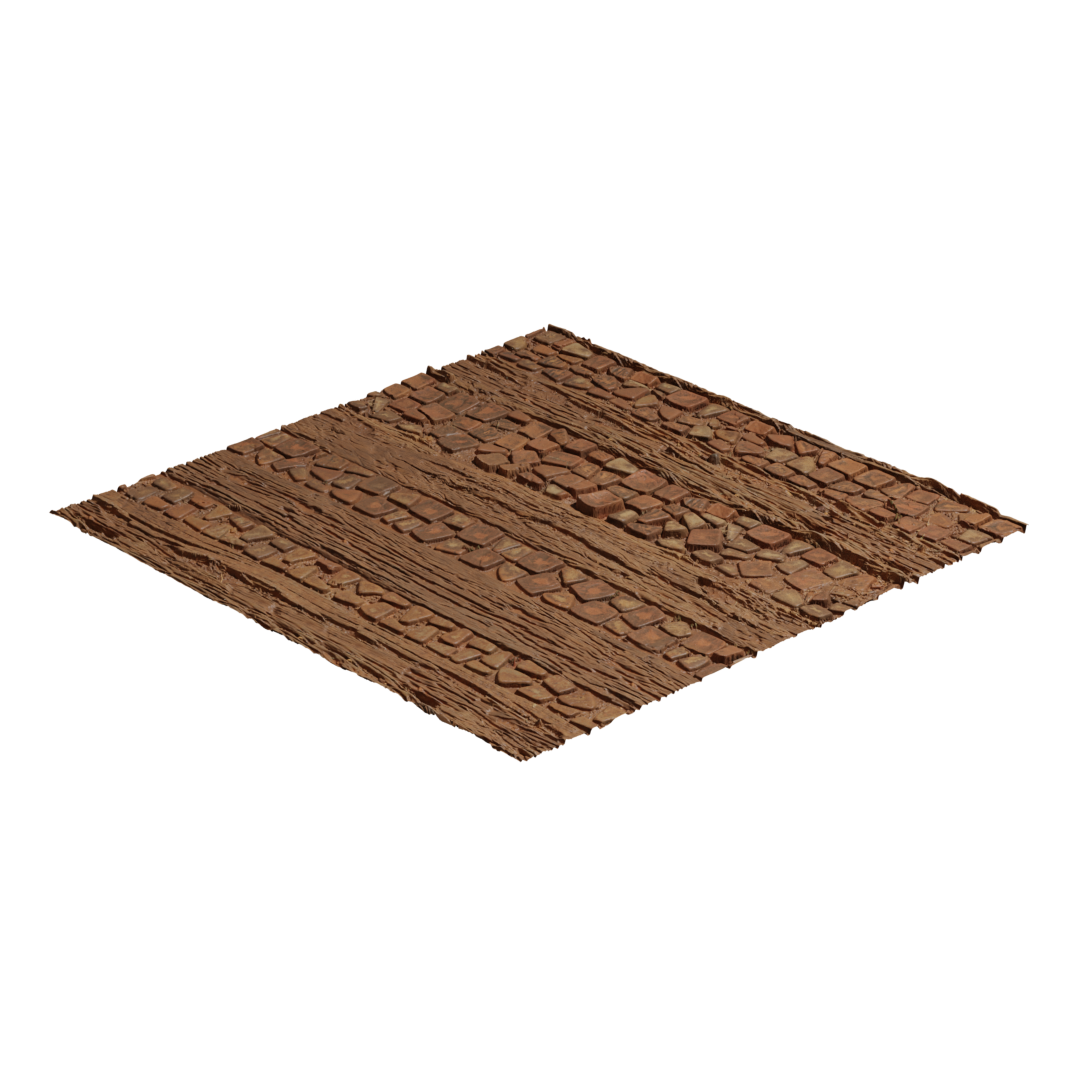
\includegraphics[scale=\myscale,scale=0.15,trim={0 8cm 0 8cm},clip]{figures/texture-wood-bump-dis1}
	
		
   \emph{Displacement}	
\end{minipage}	
\end{center}




%%%%%%%%%%%%%%%%%%%%%%%%%%%%%%%%%%%%%%%%%%%%%%%%%%%%%%%%%%%%%%%%%%%%%
\section{Appliquer une texture}

En partant d'une texture, comment l'appliquer sur l'objet réel ? Nous répondons à la question en fonction de la nature géométrique de la face des objets : triangle, rectangle, quadrilatère, cylindre ou sphère.


%--------------------------------------------------------------------
\subsection{Rectangle sur rectangle/parallélogramme}

Dans le plan, envoyer le carré unité sur un rectangle vertical est très simple. Par exemple $\Phi : (u,v) \mapsto (au,bv)$, envoie le carré $[0,1] \times [0,1]$ sur le rectangle $[0,a] \times [0,b]$. La matrice de cette application est :
$$M = \begin{pmatrix} a & 0 \\ 0 & b \end{pmatrix}.$$
Si on composait par une rotation puis une translation on pourrait obtenir n'importe quel rectangle du plan.

\myfigure{0.7}{
	\tikzinput{fig-rectangle-01}		
}

\medskip

Plus généralement si $M = \begin{pmatrix} a & b \\ c & d \end{pmatrix}\in M_2(\Rr)$ est une matrice inversible quelconque, la \defi{transformation vectorielle} associée est
$$\Phi \begin{pmatrix} u \\ v \end{pmatrix} = M \begin{pmatrix} u \\ v \end{pmatrix}$$
c'est-à-dire $\Phi(u,v)= (x,y)$ où :
$$\left\{
\begin{array}{rcl}
	x &=& au+bv \\
	y &=& cu+dv \\
\end{array}	
\right..$$

Le vecteur $\vec{i} = \left( \begin{smallmatrix} 1 \\ 0 \end{smallmatrix} \right)$ de la base canonique s'envoie sur le vecteur $\vec{p} = \left( \begin{smallmatrix} a \\ c \end{smallmatrix} \right)$
et le vecteur $\vec{j} = \left( \begin{smallmatrix} 0 \\ 1 \end{smallmatrix} \right)$ s'envoie sur le vecteur $\vec{q} = \left( \begin{smallmatrix} b \\ d \end{smallmatrix} \right)$.
Ainsi le carré unité s'envoie sur le parallélogramme engendré par $(\vec p, \vec q)$.
N'importe quel parallélogramme du plan se construit ainsi comme l'image du carré unité par une transformation vectorielle (suivie d'une translation).

\myfigure{0.7}{
	\tikzinput{fig-rectangle-02}		
}


\medskip

Dans l'espace, un parallélogramme $ABCD$ est défini par quatre points (distincts et coplanaires) tels que $\vec{AB} + \vec{AD} = \vec{AC}$.
Si on note $\vec{p} = \vec{AB} = \left( \begin{smallmatrix} x_p \\ y_p \\ z_p \end{smallmatrix} \right)$
et $\vec{q} = \vec{AD} = \left( \begin{smallmatrix} x_q \\ y_q \\ z_q \end{smallmatrix} \right)$ alors
la transformation de matrice $M \in M_{3,2}(\Rr)$ (suivie d'une translation de vecteur $\vec{OA}$) envoie le carré unité du plan sur notre parallélogramme $ABCD$ de l'espace :
$$M = \begin{pmatrix} x_p & x_q \\ y_p & y_q \\ z_p & z_q \end{pmatrix}.$$

\myfigure{0.7}{
	\tikzinput{fig-rectangle-03}		
}

Nous verrons ultérieurement comment on peut envoyer le carré unité sur un quadrilatère quelconque.
Noter cependant que $4$ points dans l'espace ne sont en général pas dans un même plan, c'est pourquoi il est beaucoup plus naturel de considérer le cas de trois points de l'espace, car trois points de l'espace sont toujours coplanaires.


%--------------------------------------------------------------------
\subsection{Coordonnées barycentriques}

\index{coordonnees@coordonnées!barycentriques}

\textbf{Triangle sur triangle.}

Le but est d'envoyer le triangle \og{}unité\fg{} du plan sur un triangle $ABC$ quelconque du plan ou de l'espace.
Cette transformation $\Phi$ doit envoyer $\vec i$ sur $\vec{AB}$ et $\vec j$ sur $\vec{AC}$.
Il existe une unique telle transformation affine $\Phi$.

\myfigure{0.8}{
	\tikzinput{fig-bary-01}		
}

Considérons $M(u,v)$ un point du triangle unité de départ. Que $(u,v)$ soient les coordonnées de $M$ signifie
$\vec{OM} = u \vec i + v \vec j$, c'est-à-dire $M = O + u \vec i + v \vec j$.
Alors $P = \Phi(M)$ où :
$$\vec{AP} = u \vec{AB} +v \vec{AC}$$
c'est-à-dire
\mybox{$P = A + u \vec{AB} + v \vec{AC}$}

\myfigure{0.8}{
	\tikzinput{fig-bary-02}		
}

Noter que ces calculs sont valables aussi bien pour $A,B,C,P$ points du plan ou de l'espace : dans tous les cas seulement deux coordonnées $u,v$ sont nécessaires.

\medskip
\textbf{Barycentre.}
Soient $A, B, C$ trois points du plan ou de l'espace.
Le point $P$ est \defi{barycentre} de $(A,\alpha)$, $(B,\beta)$, $(C,\gamma)$ (avec des réels $\alpha$, $\beta$, $\gamma$ des réels vérifiant $\alpha + \beta + \gamma \neq 0$) si :
$$\alpha \vec{PA} + \beta \vec{PB} + \gamma \vec{PC} = \vec{0}.$$
On appelle alors $(\alpha:\beta:\gamma)$ les \defi{coordonnées barycentriques} de $P$ par rapport au triangle $ABC$.
Les coordonnées sont dites \defi{normalisées} si $\alpha +\beta+\gamma = 1$.

\myfigure{0.8}{
	\tikzinput{fig-bary-03}		
}

Si $(\alpha:\beta:\gamma)$ sont des coordonnées barycentriques, alors $(\lambda \alpha : \lambda \beta : \lambda \gamma)$ le sont aussi pour tout $\lambda \in \Rr^*$ (voir les coordonnées homogènes du chapitre \og{}Transformations de l'espace\fg{}).
Ainsi par multiplication par un facteur $\lambda = \frac{1}{\alpha+\beta+\gamma}$ on peut toujours se ramener à des coordonnées barycentriques normalisées.


\medskip
\textbf{Exemples.}

\myfigure{0.8}{
	\tikzinput{fig-bary-04}		
}


Les calculs avec les coordonnées barycentriques sont pratiques : le milieu de deux points $P(\alpha:\beta:\gamma)$
et $Q(\alpha':\beta':\gamma')$ est $\frac{P+Q}{2}$ de coordonnées barycentriques $(\frac{\alpha+\alpha'}{2}:\frac{\beta+\beta'}{2} :\frac{\gamma+\gamma'}{2})$.

L'\defi{isobarycentre} $G$ de $A, B, C$ est $G = \frac{A+B+C}{3}$ et a pour coordonnées barycentriques $(\frac13:\frac13:\frac13) = (1:1:1)$.
Il vérifie $\vec{GA} + \vec{GB} + \vec{GC} = \vec{0}$.

Quelque remarques sur les coordonnées barycentriques normalisées ($\alpha+\beta+\gamma=1$).
\begin{itemize}
	\item Intuitivement, plus $P(\alpha:\beta:\gamma)$ est proche de $A$, plus $\alpha$ est grand ; plus $P$ est proche de $B$, plus $\beta$ est grand ; plus $P$ est proche de $C$, plus $\gamma$ est grand.
	\item $P$ est situé dans le triangle $ABC$ si et seulement si $\alpha\ge0$, $\beta\ge0$ et $\gamma\ge0$.
	\item $P$ est situé sur la droite $(BC)$ si et seulement si $\alpha=0$.
\end{itemize}

\myfigure{0.6}{
	\tikzinput{fig-bary-05}		
}

\medskip
\textbf{Aires.}

On peut déterminer géométriquement les coordonnées barycentriques $(\alpha:\beta:\gamma)$ d'un point $P$.
Chaque coefficient est égal à l'aire du triangle opposé divisée par l'aire du triangle total :
$$\alpha = \frac{\mathcal{A}_{\triangle}(PBC)}{\mathcal{A}_{\triangle}(ABC)}
\qquad
\beta = \frac{\mathcal{A}_{\triangle}(PCA)}{\mathcal{A}_{\triangle}(ABC)}
\qquad
\gamma = \frac{\mathcal{A}_{\triangle}(PAB)}{\mathcal{A}_{\triangle}(ABC)}$$



\myfigure{0.8}{
	\tikzinput{fig-bary-06}		
}


Ces formules sont valables pour un point $P$ à l'intérieur du triangle. Nous verrons la preuve de ces formules un peu plus tard.
On rappelle que l'on calcule facilement l'aire (sans signe) d'un triangle à l'aide des formules suivantes :
$$\mathcal{A}_{\triangle} (ABC) 
= \frac12 \| \vec{AB} \wedge \vec{AC} \|$$
Cette formule est valable dans le plan et l'espace.
Dans le plan uniquement on a aussi :
$$\mathcal{A}_{\triangle} (ABC) = \frac12 \left| \det(\vec{AB}, \vec{AC}) \right|$$



%--------------------------------------------------------------------
\subsection{Conversions}
\medskip
\textbf{Passage de $(u,v)$ à $(\alpha:\beta:\gamma)$.}

Il y a $3$ coordonnées barycentriques $\alpha$, $\beta$, $\gamma$, mais comme elles sont définies à un facteur multiplicatif $\lambda$ près, il y a seulement deux degrés de liberté.

\begin{proposition}
	\sauteligne
	\begin{itemize}
		\item Si $P = A +  u \vec{AB} + v \vec{AC}$ alors $P$ a pour coordonnées barycentriques $(1-u-v:u:v)$.
		\item Réciproquement, si $P$ a pour coordonnées barycentriques $(\alpha:\beta:\gamma)$ alors 
		$P = A +  u \vec{AB} + v \vec{AC}$ avec $u = \frac{\beta}{\alpha+\beta+\gamma}$ et $v = \frac{\gamma}{\alpha+\beta+\gamma}$.
	\end{itemize}
\end{proposition}

\begin{proof}
La preuve c'est une reformulation de l'écriture $P = A +  u \vec{AB} + v \vec{AC}$ sous la forme
$\vec{PA} + u \vec{AB} + v \vec{AC} = \vec{0}$.
On décompose $\vec{AB} = \vec{AP} + \vec{PB}$ et $\vec{AC} = \vec{AP} + \vec{PC}$ pour obtenir
$(1-u-v)\vec{PA} + u \vec{PB} + v \vec{PC} = \vec{0}$.
\end{proof}


\medskip
\textbf{Passage de $(u,v)$ à $(x,y)$.}

Nous avons deux façons de repérer un point $P$ du plan ou de l'espace, d'une part les coordonnées cartésiennes $(x,y)$ ou $(x,y,z)$ et d'autre part les coordonnées $(u,v)$ associées aux coordonnées barycentriques $(1-u-v:u:v)$.
Voici comment passer de l'une à l'autre.
\begin{proposition}
	\sauteligne
\begin{enumerate}
	\item Dans le plan 
	$$\begin{pmatrix} x \\ y \end{pmatrix} = T_2  \begin{pmatrix} u \\ v \end{pmatrix} + \begin{pmatrix} x_A \\ y_A \end{pmatrix} \qquad \qquad  \begin{pmatrix} u \\ v \end{pmatrix} = T_2^{-1}  \begin{pmatrix} x -x_A \\ y-y_A \end{pmatrix}$$
	où 
	$$T_2 = \begin{pmatrix} x_B-x_A & x_C-x_A \\ y_B-y_A & y_C-y_A \end{pmatrix}.$$

	\item Dans l'espace 
	$$\begin{pmatrix} x \\ y \\ z \end{pmatrix} = T_3  \begin{pmatrix} u \\ v \end{pmatrix} + \begin{pmatrix} x_A \\ y_A \\ z_A \end{pmatrix}\qquad \text{ où } \qquad
    T_3 = \begin{pmatrix} x_B-x_A & x_C-x_A \\ y_B-y_A & y_C-y_A  \\ z_B-z_A & z_C-z_A \end{pmatrix}.$$	
    On a  
    $$\begin{pmatrix} u \\ v \end{pmatrix} = T_2^{-1}  \begin{pmatrix} x -x_A \\ y-y_A \end{pmatrix}$$
    où $T_2$ est la matrice du cas précédent.
\end{enumerate}
\end{proposition}	

\begin{proof}
Il s'agit encore une fois juste de l'écriture de l'égalité $P = A +  u \vec{AB} + v \vec{AC}$ en coordonnées cartésiennes.
\end{proof}

On sait que si $M = \begin{pmatrix} a & b \\ c & d \end{pmatrix}$ est inversible alors 
$$M^{-1} = \frac1{\det M} \begin{pmatrix} d & -b \\ c & a \end{pmatrix}$$
où 
$$\det M = \begin{vmatrix} a & b \\ c & d \end{vmatrix} = ad-bc.$$
On rappelle que $\det(M)$ est l'aire (avec signe) du parallélogramme formé par $\vec p = \begin{pmatrix} a \\ c \end{pmatrix}$ et $\vec q = \begin{pmatrix} b \\ d \end{pmatrix}$. Autrement dit c'est le double de l'aire du triangle. Ainsi $\mathcal{A}_{\triangle} = \frac12 \det(M)$.
 
\myfigure{0.8}{
	\tikzinput{fig-rectangle-04}		
}
 
Intéressons-nous au calcul :
$\begin{pmatrix} u \\ v \end{pmatrix} = T_2^{-1}  \begin{pmatrix} x -x_A \\ y-y_A \end{pmatrix}$.
On obtient alors 
$$u 
= \frac{\begin{vmatrix}x-x_A & x_C-x_A \\ y-y_A & y_C-y_A\end{vmatrix}}
       {\begin{vmatrix}x_B-x_A & x_C-x_A \\ y_B-y_A & y_C-y_A\end{vmatrix}} 
= \frac{\mathcal{A}_{\triangle}(\vec{AP},\vec{AC})}
        {\mathcal{A}_{\triangle}(\vec{AB},\vec{AC})} 
\qquad \text{ et } \qquad 
v 
= \frac{\begin{vmatrix}x_B-x_A & x-x_A \\ y_B-y_A & y-y_A\end{vmatrix}}
{\begin{vmatrix}x_B-x_A & x_C-x_A \\ y_B-y_A & y_C-y_A\end{vmatrix}} 
= \frac{\mathcal{A}_{\triangle}(\vec{AB},\vec{AP})}
{\mathcal{A}_{\triangle}(\vec{AB},\vec{AC})} 
$$
Ce sont les formules des coordonnées barycentriques calculées avec des aires de triangles comme on l'avait annoncé plus haut.
		
		
%%%%%%%%%%%%%%%%%%%%%%%%%%%%%%%%%%%%%%%%%%%%%%%%%%%%%%%%%%%%%%%%%%%%%
\section{Autres figures géométriques}

%--------------------------------------------------------------------
\subsection{Répétitions}

Si la face à décorer est grande, il peut être utile de réaliser la texture par répétitions d'un motif de base. 

\myfigure{1.2}{
	\tikzinput{fig-repeter-00}		
}

Voici plusieurs façons d'étendre un motif :
\begin{itemize}
	\item \emph{répétition} : le motif de base est répété par translations,
	\item \emph{miroir} : le motif de base est répété par symétries axiales,
	\item \emph{bord} : on entoure le motif d'une couleur neutre, pour éviter les problèmes au bord de la face lors de l'application de la texture,
	\item \emph{extension/\emph{clamp}} : on étend le motif en rajoutant une bande de sécurité tout autour du motif (cette bande n'est pas sensé servir au-delà d'une largeur d'un pixel), c'est encore une fois pour éviter les problèmes de bord.
\end{itemize}

\myfigure{0.7}{
	\tikzinput{fig-repeter-01}\quad
	\tikzinput{fig-repeter-02}\quad
	\tikzinput{fig-repeter-03}\quad
	\tikzinput{fig-repeter-04}\quad			
}

%--------------------------------------------------------------------
\subsection{Pixel le plus proche}


Jusqu'à présent nous avons présenté le texturage avec des calculs exacts où $(u,v) \in [0,1]^2$ et 
 $(x,y,z) \in \Rr^3$. 
Mais dans la pratique on travaille avec des coordonnées qui correspondent à des pixels.
On rappelle comment se déroule le texturage inverse : pour colorier le point $(x,y,z)$ d'un objet, on lui associe les coordonnées réelles $(u,v) \in [0,1]^2$ et on le colorie selon la couleur $\mathcal{C}(u,v)$. 

\myfigure{0.7}{
	\tikzinput{fig-texture-pixels-01}		
}


Mais comment concrètement décider ce qu'est $\mathcal{C}(u,v)$ à partir d'une image définissant la texture ?

\textbf{Pixel le plus proche.}
Considérons une image carrée de taille $N\times N$ pixels, on note $(i,j)$ avec $0 \le i,j < N$ les coordonnées des centres des pixels. Identifions cette même image avec le carré unité $[0,1]^2$ de coordonnées $(u,v)$. Noter que les origines de ces deux systèmes de coordonnées sont différentes.

\myfigure{0.7}{
	\tikzinput{fig-texture-pixels-02}		
}

Au centre $(i,j)$ d'un pixel on associe les réels 
$$(u,v) = \left(\frac{i+\frac12}{N}, \frac{j+\frac12}{N} \right)\in [0,1]^2$$

\myfigure{0.7}{
	\tikzinput{fig-texture-pixels-03}		
}


Dans l'autre sens, c'est plus délicat, puisque $(u,v)$ ne correspond généralement pas au centre d'un pixel.
On envoie donc $(u,v)$ sur le centre du pixel le plus proche :
$$(i,j) = \left( \lfloor Nu \rfloor, \lfloor Nv \rfloor \right)$$
(sauf si $u=1$ auquel cas $i=N-1$ ou $v=1$ auquel cas $j=N-1$).
On rappelle que $\lfloor x \rfloor$ désigne la partie entière de $x$.

Ce choix pose plusieurs problèmes.

D'une part si la texture est petite (elle a très peu de pixels) par rapport à la face de l'objet à colorier, alors le rendu sera de mauvaise qualité et fera apparaître une pixellisation.

\myfigure{0.8}{
	\tikzinput{fig-texture-pixels-04}		
}


D'autre part peuvent apparaître des problèmes d'échantillonage pour des grandes textures périodiques.

\myfigure{0.8}{
	\tikzinput{fig-texture-pixels-05}		
}


%--------------------------------------------------------------------
\subsection{Interpolation bilinéaire}

\index{interpolation!bilineaire@bilinéaire}

Pour éviter les problèmes précédents, il est raisonnable de tenir compte de la couleur de plusieurs pixels proches et pas seulement de celui le plus près. L'interpolation bilinéaire tient compte des $4$ pixels les plus proches.

De façon générale considérons une fonction $F(x,y)$ qui pour l'instant est définie uniquement pour des valeurs entières, c'est-à-dire on connaît $F(x_i,y_j)$ pour $x_i, y_j \in \Zz$.
Comment interpoler une valeur pour $F(x,y)$ avec $(x,y) \in \Rr^2$ ?

On note $(x_1,y_1)$, $(x_1,y_2)$, $(x_2,y_1)$, $(x_2,y_2)$ les sommets à coordonnées entières du carré qui entoure $(x,y)$.
On note $x' = x-x_1$ et $y' = y-y_1$. Alors l'\defi{interpolation bilinéaire} de $F$ est définie par :
\begin{align*}
F(x,y) & = (1-x')(1-y')F(x_1,y_1) \\
       & \quad +  (1-x')y'F(x_1,y_2) \\
       & \quad\quad +  x'(1-y')F(x_2,y_1) \\
       & \quad\quad\quad +  x'y'F(x_2,y_2)
\end{align*}


\myfigure{0.8}{
	\tikzinput{fig-texture-pixels-06}		
}
      
Le coefficient associé à $F(x_1,y_1)$ est l'aire du rectangle opposé à ce sommet. De même pour les autres coefficients. Ainsi plus $(x,y)$ est proche d'un sommet, plus la valeur en ce sommet a d'importance.

\myfigure{0.8}{
	\tikzinput{fig-texture-pixels-07}		
}

Revenons à nos pixels, pour un point $(u,v) \in [0,1]^2$ du carré unité, on lui associe les coordonnées réelles $(x,y) = ( N(u+\frac12) , N(v+\frac12) )$ de l'image. On note $(x_1,y_1) = (\lfloor x \rfloor, \lfloor y \rfloor )$. Puis on pose $x_2=x_1+1$ et $y_2=y_1+1$.

Reprenons notre exemple d'une image $2 \times 2$ (à gauche ci-dessous), l'interpolation bilinéaire permet de la transformer en une image $4\times 4$.


\begin{center}
		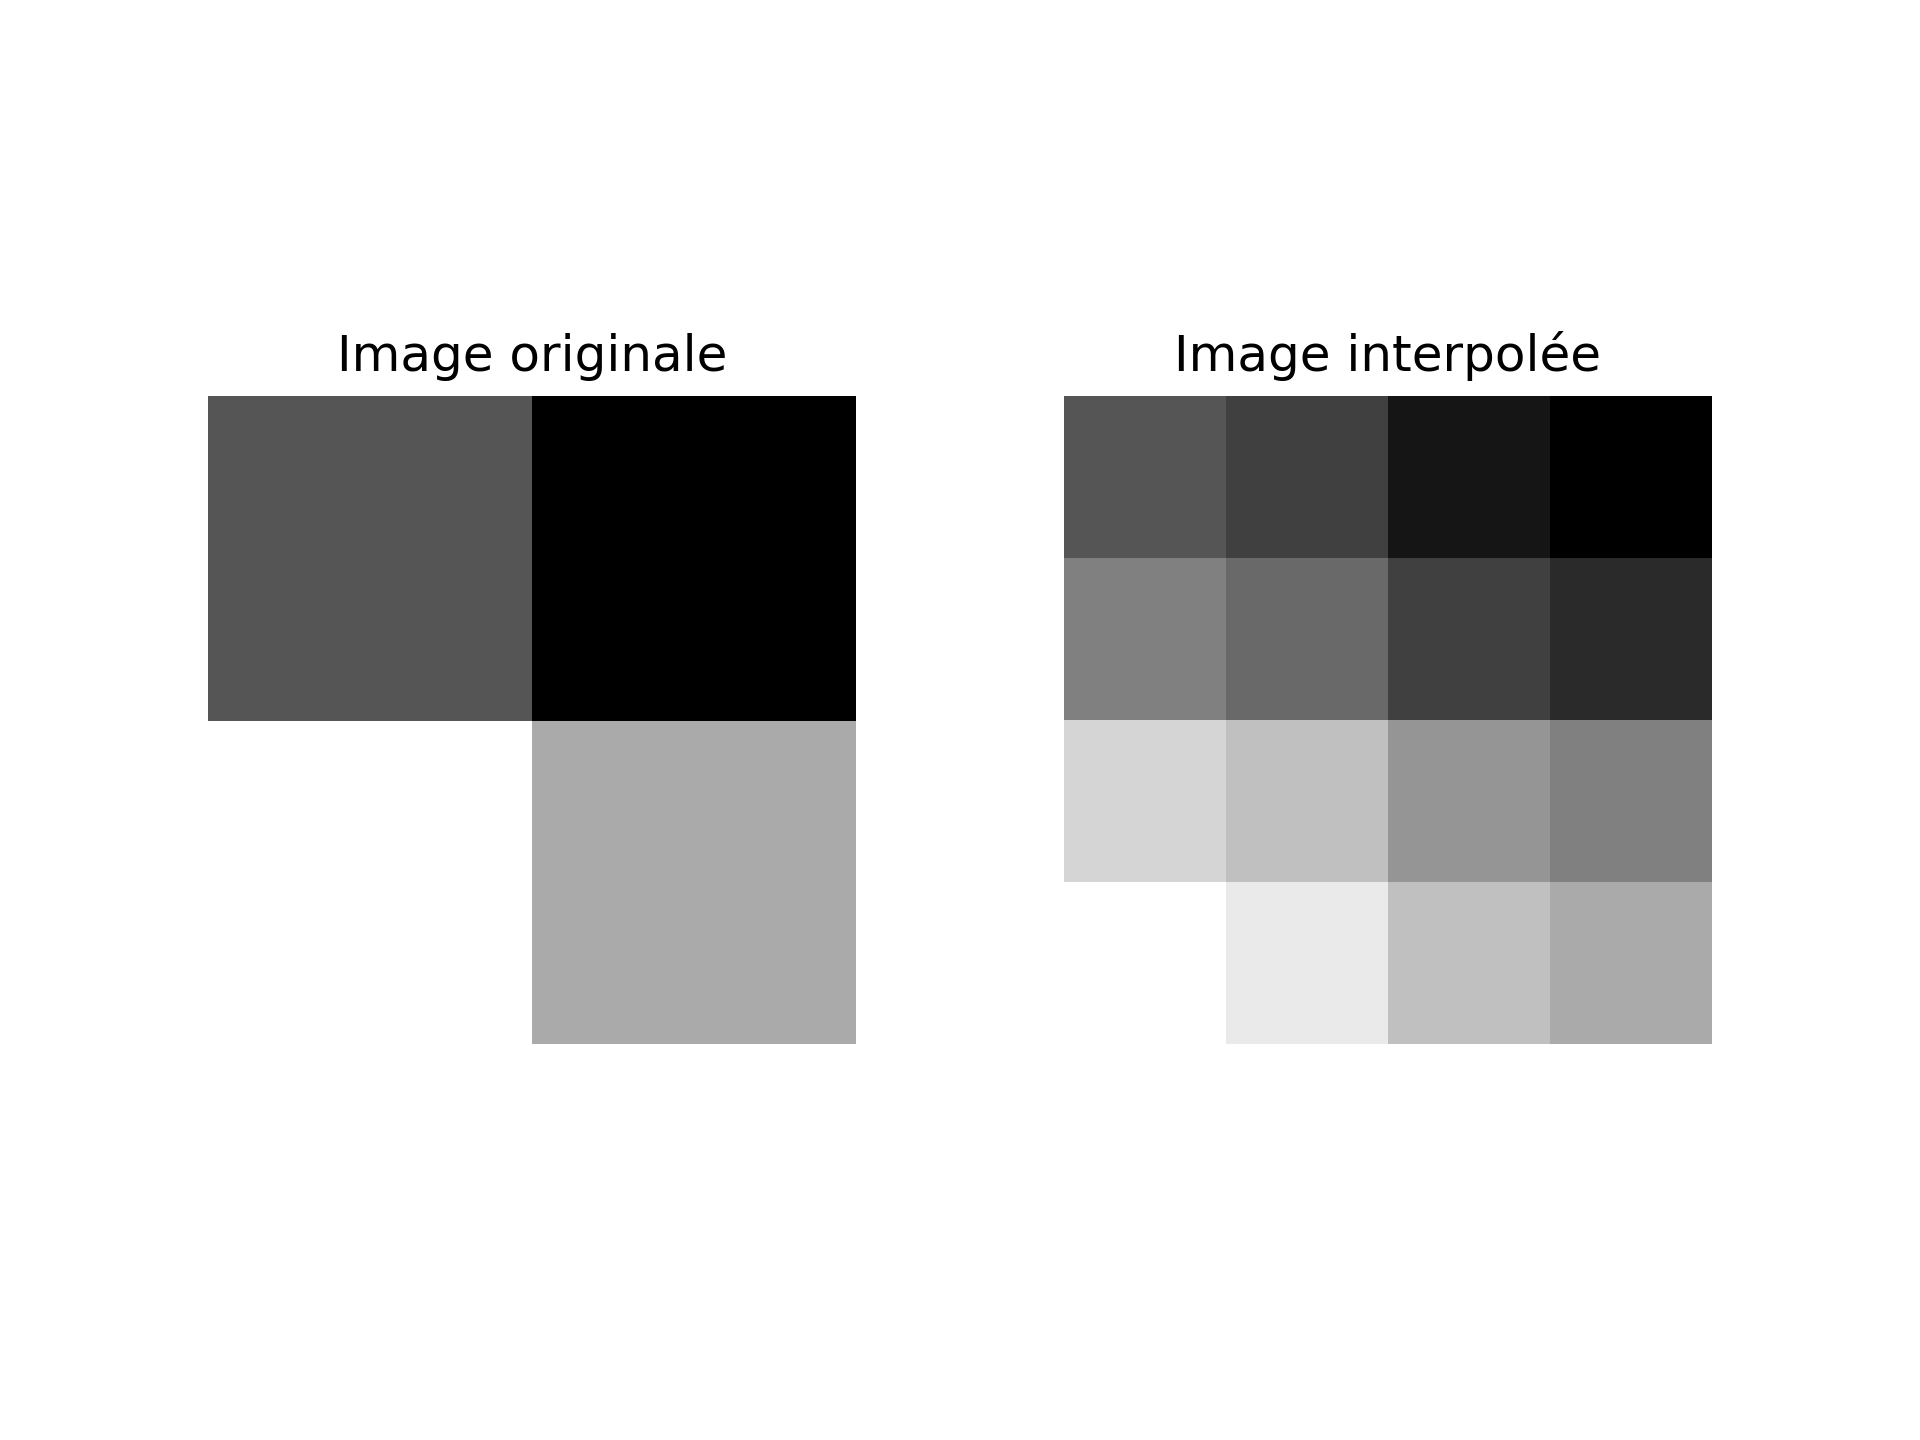
\includegraphics[scale=\myscale,scale=0.7]{figures/interpolation_bilineaire_1}  
\end{center}

L'interpolation bilinéaire permet un agrandissement artificiel d'une image.
Considérons une image (à gauche), on zoome sur une petite portion d'image qui apparaît alors pixelisée (au centre), l'interpolation bilinéaire permet d'obtenir une image plus lisse (à droite).
\begin{center}
	\begin{minipage}{0.32\textwidth}
	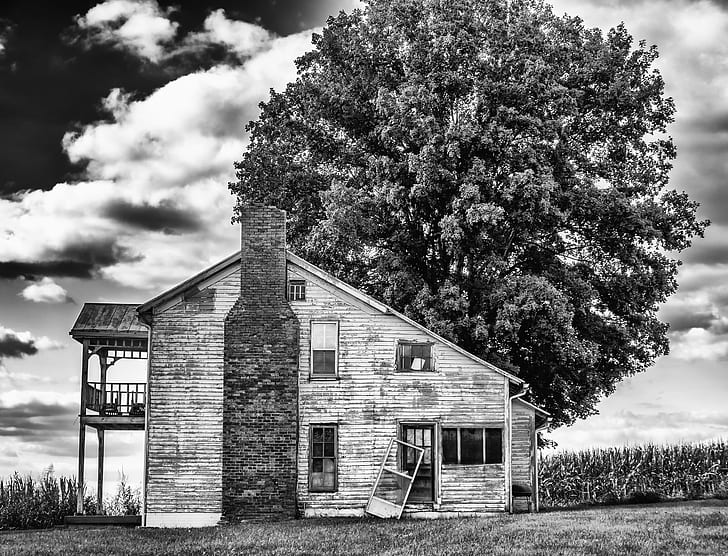
\includegraphics[scale=\myscale,scale=0.22]{figures/image_maison} 
	\end{minipage} 
	\begin{minipage}{0.66\textwidth}
	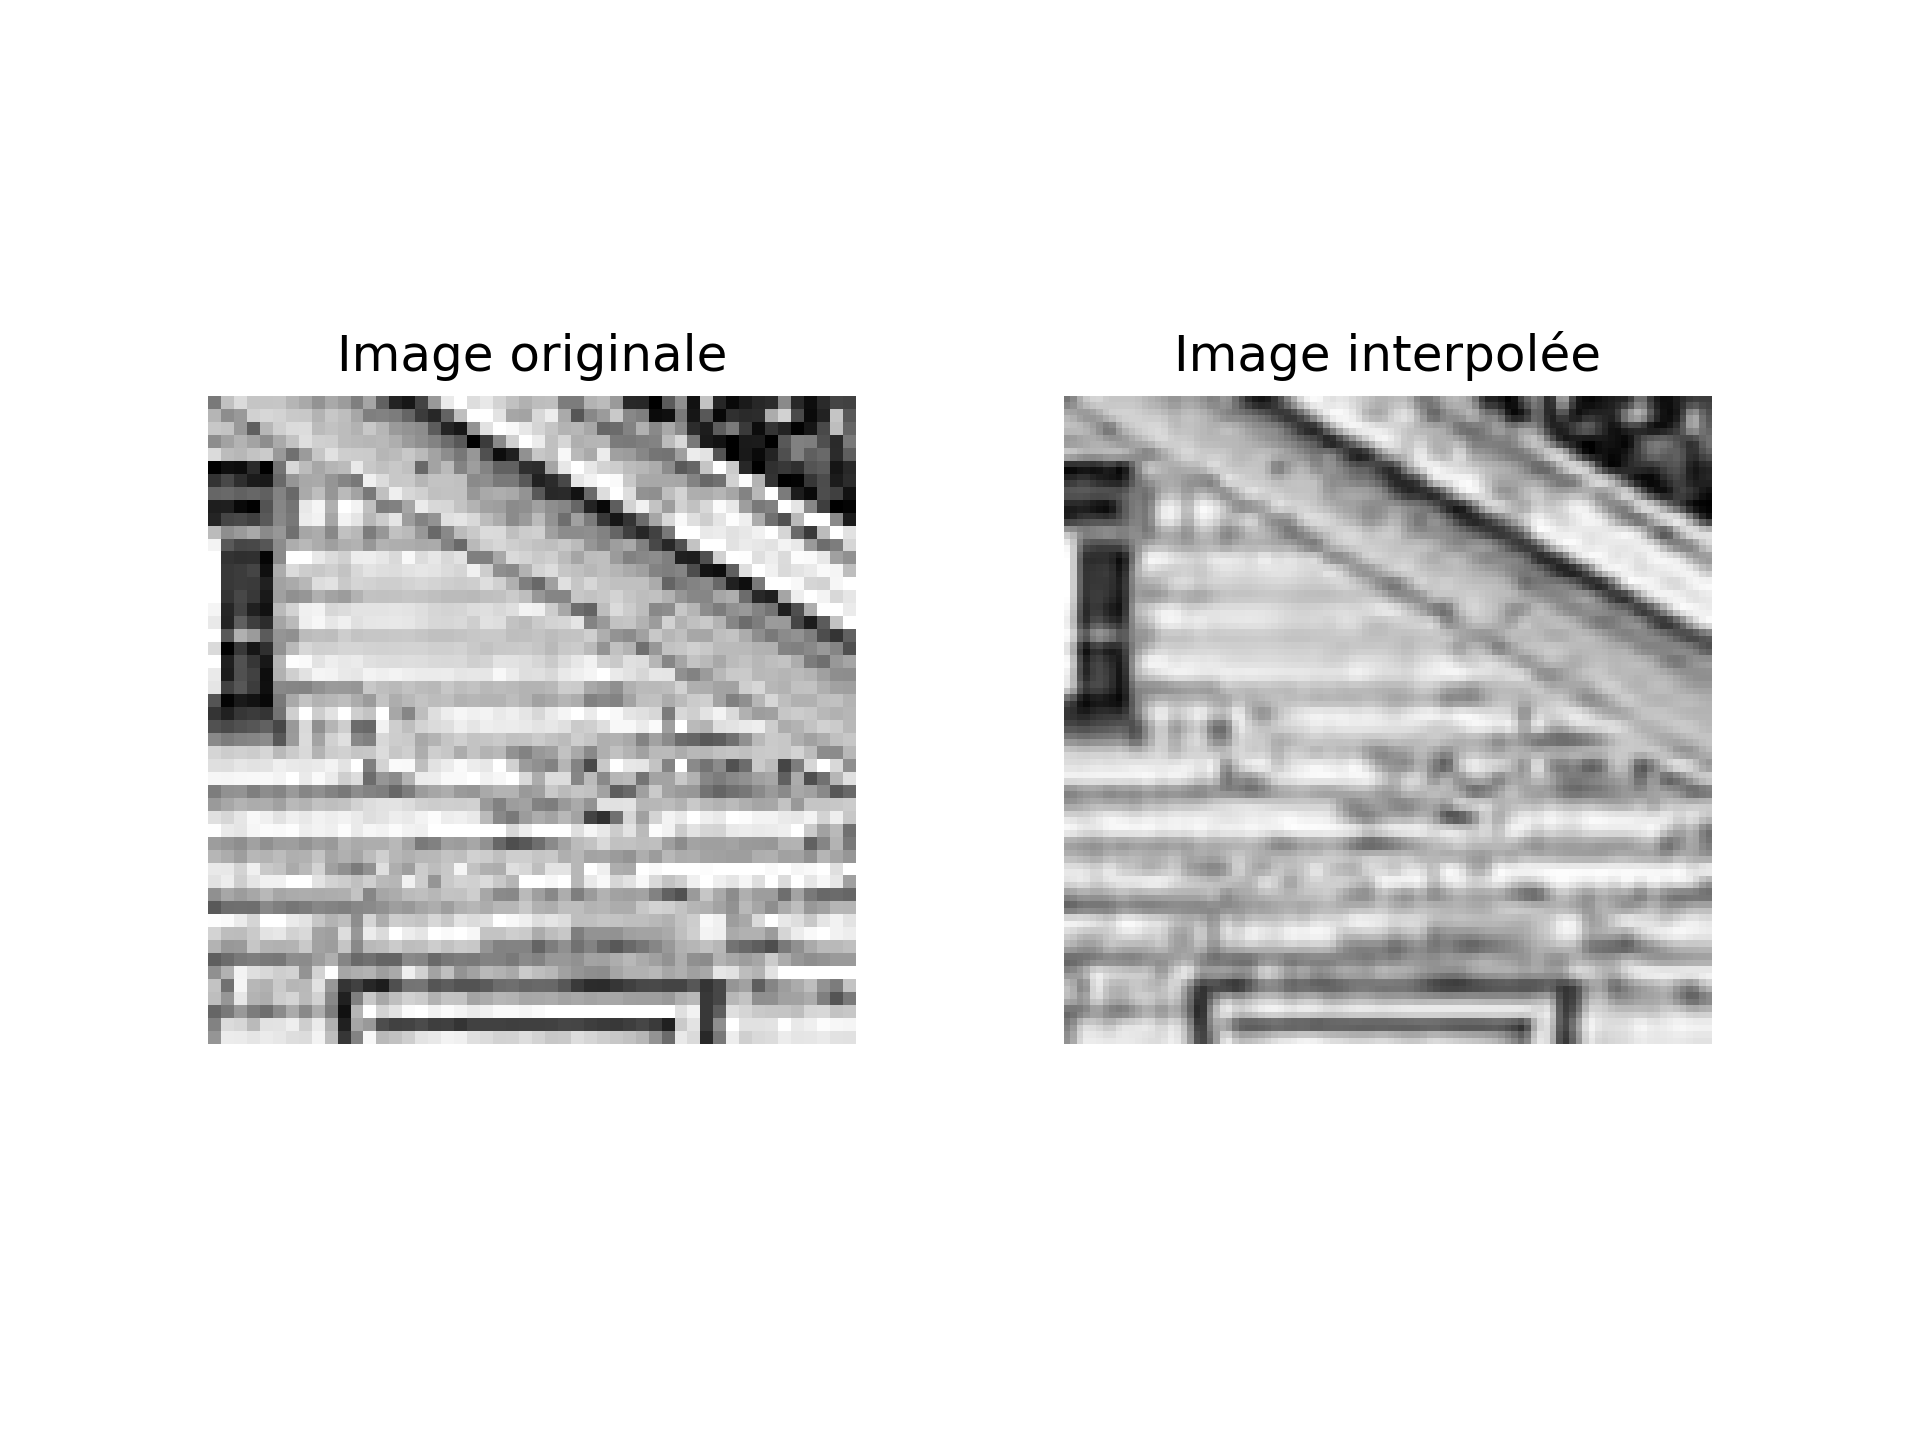
\includegraphics[scale=\myscale,scale=0.8,trim={0 2cm 0 2cm},clip]{figures/interpolation_bilineaire_2}  
	\end{minipage}
\end{center}

Bien sûr on pourrait faire mieux avec plus de pixels. Par exemple l'interpolation bicubique prend en compte une moyenne calculée sur les $16$ pixels voisins. Mais les calculs sont longs et pas applicables à un rendu en temps réel.


%--------------------------------------------------------------------
\subsection{Quadrilatère}

Le maillage des objets 3D est souvent réalisé par des triangulations. 
Mais il peut être plus adapté d'utiliser un maillage qui contient des quadrilatères.
Un \defi{quadrilatère} (\emph{quad}) de l'espace, ce sont $4$ points coplanaires (le quadrilatère est généralement supposé convexe).

\myfigure{0.8}{	
	\tikzinput{fig-quadrilatere-01}
}

Imaginez que vous êtes dans une rue entourée de deux murs, ces deux murs sont des rectangles de l'espace, mais ce que vous voyez en perspective ce sont des quadrilatères.
Représenter ce mur est donc lié à la vision d'un objet (ici un rectangle) dans l'espace et a été traité en détail dans le chapitre \og{}Perspective\fg{}. Cependant notre texture elle n'est pas un objet de l'espace. Il faut donc explicitement décrire l'application $\varphi$ qui permet de décorer ce mur (qui est un quadrilatère à l'écran).

\myfigure{0.8}{
	\tikzinput{fig-quadrilatere-03}
}
Le problème se ramène donc à envoyer notre carré unité $[0,1]^2$ sur un quadrilatère convexe $ABCD$ quelconque du plan.

\myfigure{0.8}{
	\tikzinput{fig-quadrilatere-02}
}

\medskip
\textbf{Interpolation bilinéaire.}
On considère le carré unité $A_0B_0C_0D_0$ de coordonnées $(u,v) \in [0,1]^2$.
Soit un quadrilatère convexe $ABCD$. L'interpolation bilinéaire qui envoie 
le carré sur le quadrilatère est :
\begin{align*}
\varphi(u,v)  
& = (1-u)(1-v) A  \\
& \quad +  u(1-v) B \\
& \quad\quad +   uv C \\
& \quad\quad\quad +  (1-u)v D
\end{align*}

\myfigure{0.8}{
	\tikzinput{fig-quadrilatere-04}
}

Dans ces calculs on identifie les points avec des vecteurs (ou bien leurs coordonnées) $A(x_A,y_A)$,\ldots{}
C'est l'interpolation bilinéaire précédente (en faisant bien attention aux coefficients associés à chaque sommet). Les calculs sont très faciles. Comme son nom l'indique cette fonction est linéaire dans les deux directions : un segment vertical du carré est envoyé sur un segment inclus dans le quadrilatère, un segment horizontal aussi. Par contre cette représentation du quadrilatère ne correspond pas exactement à la réalité d'un carré vu en perspective.

\myfigure{1}{
	\tikzinput{fig-quadrilatere-05}
}


\medskip
\textbf{Transformation projective.}

La fonction qui envoie un carré sur un quadrilatère et qui correspond à la perspective linéaire 
s'appelle une homographie du plan.
Une \defi{homographie}\index{homographie} (ou \defi{transformation projective}) est une application
$\varphi$ de $\Rr^2$ dans $\Rr^2$ définie par $\varphi : (u,v) \mapsto (x,y)$ où :
$$x = \frac{a_0+a_1u+a_2v}{1+c_1u+c_2v}
\qquad\qquad
y = \frac{b_0+b_1u+b_2v}{1+c_1u+c_2v}$$
avec $8$ coefficients réels $a_0$, $a_1$, $a_2$, $b_0$, $b_1$,$b_2$, $c_1$ et $c_2$. (Noter que les deux dénominateurs de $x$ et $y$ sont identiques.)

Notons le carré unité $[0,1]^2$ par $A_0B_0C_0D_0$ (en fait cela pourrait être un quadrilatère quelconque). Soient $A$, $B$, $C$, $D$ quatre points du plan (formant aussi un quadrilatère). Alors il existe une unique homographie $\varphi$ telle que :
$$\varphi(A_0) = A \qquad \varphi(B_0) = B \qquad \varphi(C_0) = C \qquad \varphi(D_0) = D.$$

Comment déterminer cette homographie ? Il faut déterminer les $8$ coefficients, pour cela nous avons $4$ conditions :
$\varphi(0,0) = (x_A,y_A)$, 
$\varphi(1,0) = (x_B,y_B)$,
$\varphi(0,1) = (x_D,y_D)$,
$\varphi(1,1) = (x_C,y_C)$.
Chacune de ces conditions  fournit deux équations. Par exemple $\varphi(1,0) = (x_B,y_B)$ s'écrit (en posant $u=1$, $v=0$) : $x_B = \frac{a_0+a_1}{1+c_1}$ et $y_B = \frac{b_0+b_1}{1+c_1}$.
En multipliant par le dénominateur on obtient $8$ équations linéaires du type
$$(1+c_1u+c_2v)x = a_0+a_1u+a_2v
\qquad\text{ ou }\qquad
(1+c_1u+c_2v)y = b_0+b_1u+b_2v$$
où les inconnues sont les $8$ coefficients $a_0,a_1,\ldots,c_2$ et les données sont les $x$ parcourant $\{x_A, x_B, x_C, x_D\}$ et $y$  parcourant $\{y_A, y_B, y_C, y_D\}$.

Nous obtenons donc un système de $8$ équations linéaires avec $8$ inconnues, qui admet une unique solution (sauf exceptions que l'on ne discutera pas ici). Résoudre ce système revient à inverser une matrice $8\times8$ (avec beaucoup de $0$) ce qui est facile pour un ordinateur.
Notons :
$$M = \begin{pmatrix}
1 & 0 & 0 & 0 & 0 & 0 & 0 & 0 \\
0 & 0 & 0 & 1 & 0 & 0 & 0 & 0 \\
1 & 1 & 0 & 0 & 0 & 0 & -x_B & 0 \\
0 & 0 & 0 & 1 & 1 & 0 & -y_B & 0 \\
1 & 1 & 1 & 0 & 0 & 0 & -x_C & -x_C \\
0 & 0 & 0 & 1 & 1 & 1 & -y_C & -y_C \\
1 & 0 & 1 & 0 & 0 & 0 & 0 & -x_D \\
0 & 0 & 0 & 1 & 0 & 1 & 0 & -y_D \\	
\end{pmatrix}
\qquad 
H = \begin{pmatrix}
a_0 \\ a_1 \\ a_2 \\ b_0 \\ b_1 \\ b_2 \\ c_1 \\ c_2	
\end{pmatrix}
\qquad
Q = \begin{pmatrix}
x_A \\ y_A \\ x_B \\ y_B \\ x_C \\ y_C \\ x_D \\ y_D 	
\end{pmatrix}
$$
Le système d'équations est $MH = Q$, ainsi on obtient les coefficients $H$ de l'homographie en fonction des coordonnées $Q$ du quadrilatère par :
$$H = M^{-1} Q.$$


\medskip
\textbf{Exemple.}
Sur la figure ci-dessous les sommets du quadrilatère $ABCD$ ont pour coordonnées :
$(2,-1)$, $(4,-\frac12)$, $(5,1)$, $(3,2)$, qui forment le vecteur 
$Q = (2,-1, 4,-\frac12, 5,1, 3,2)$.
On trouve $H = (a_0, a_1, a_2, b_0, b_1, b_2, c_1, c_2) = (2, 5, -0.125, -1, 0.125,  2.25, 0.75, -0.375)$ et donc les équations définissant $\varphi$. 
On peut voir le quadrilatère\couleurnb{ bleu}{} comme un carré vu en perspective.
 
Le calcul
\begin{center}
	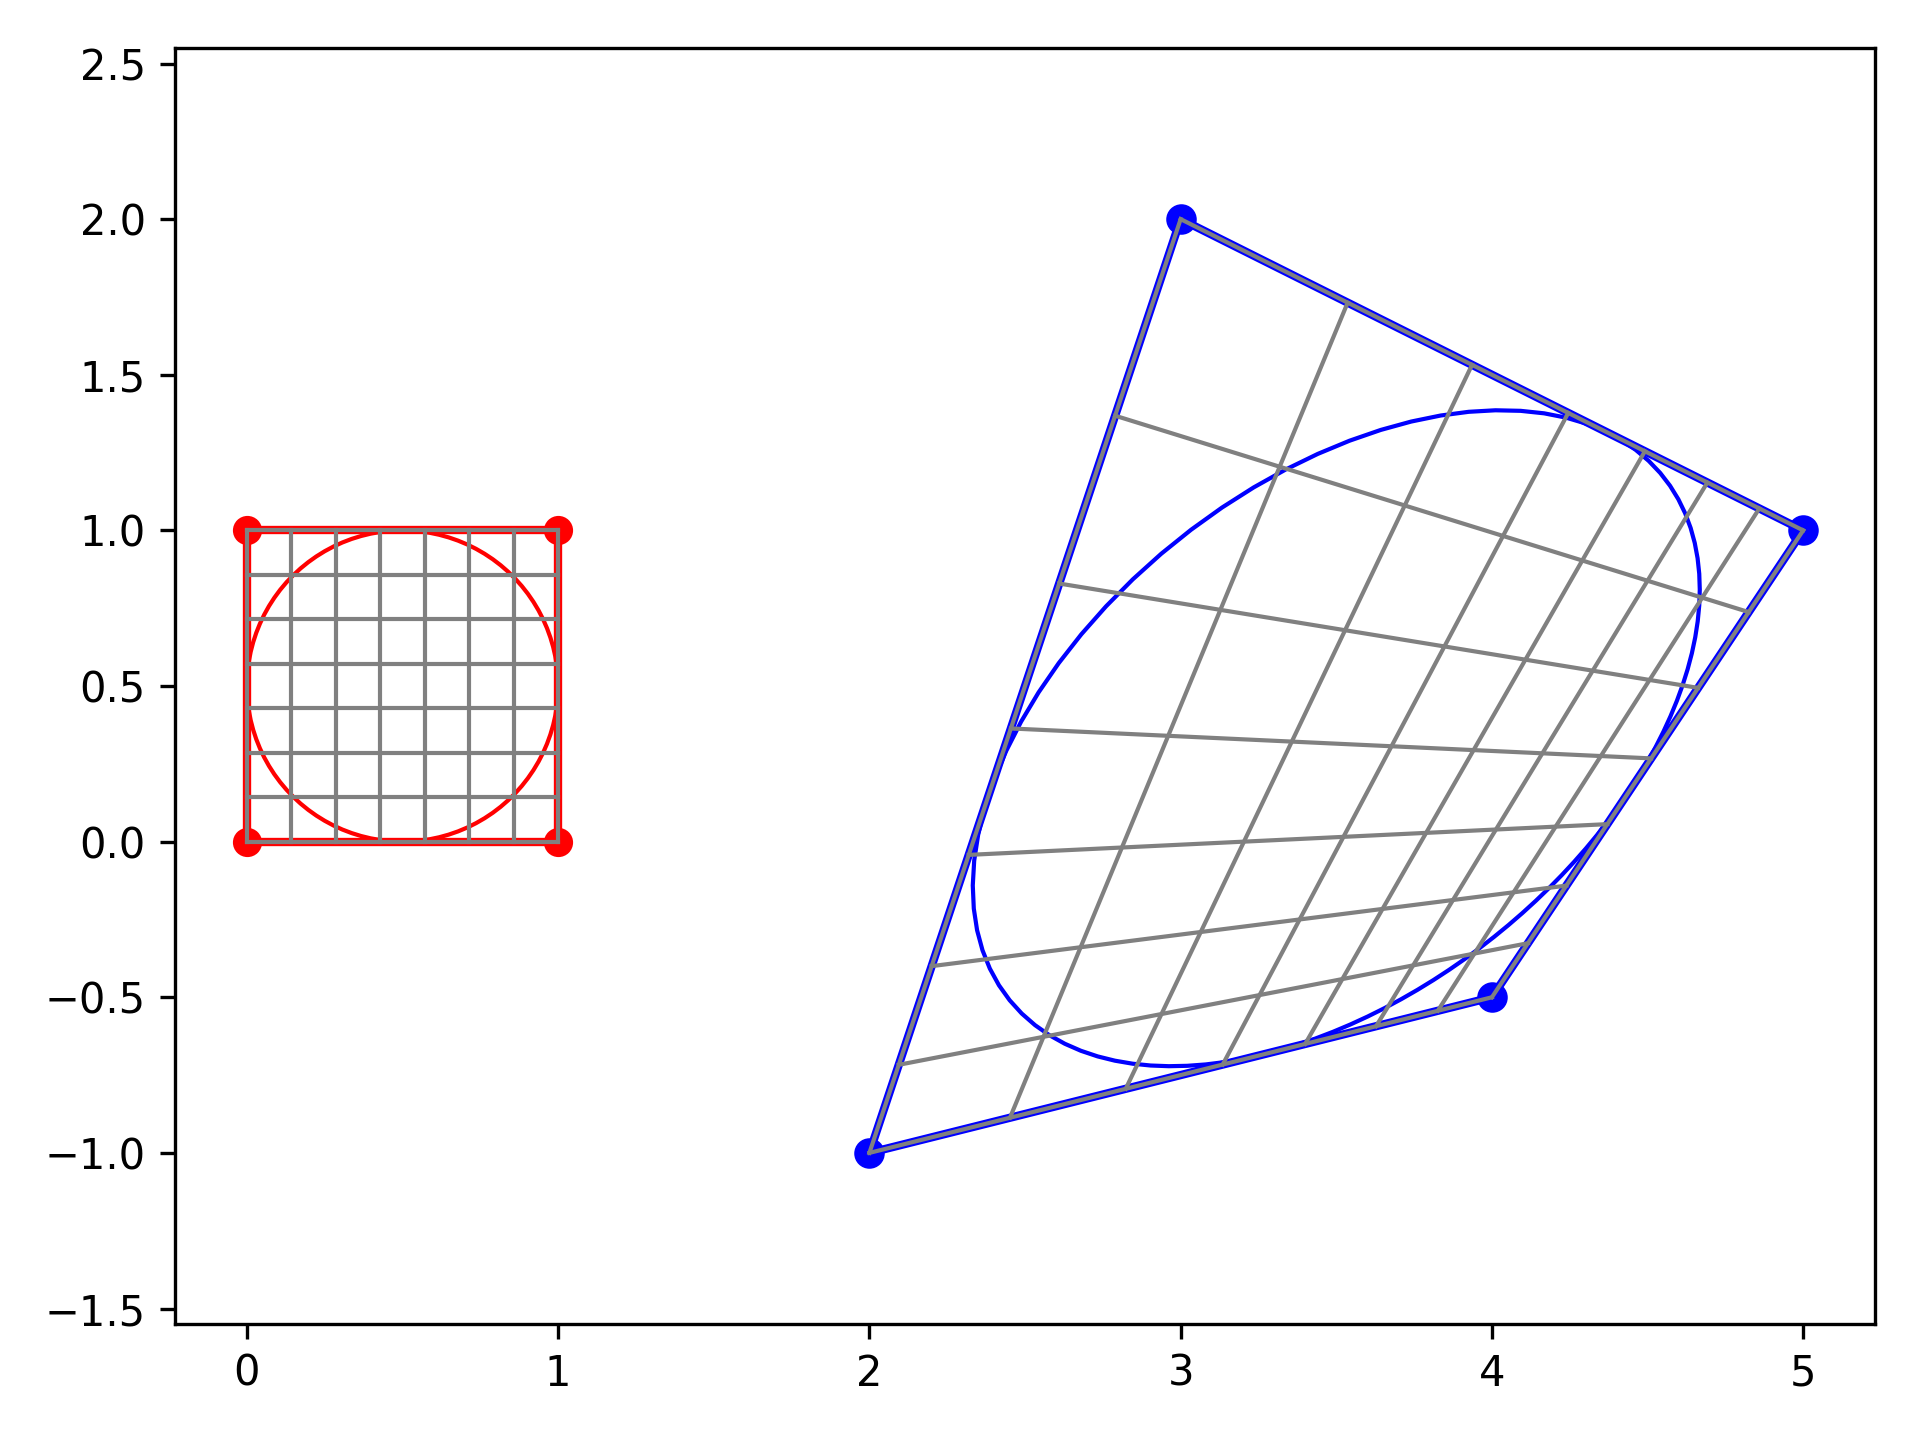
\includegraphics[scale=\myscale,scale=0.7]{figures/carre-quadrilatere}
\end{center}


\medskip

Une façon plus efficace pour les calculs serait d'utiliser les coordonnées homogènes (voir le chapitre \og{}Transformations de l'espace\fg{}). On rappelle qu'un point $(x,y) \in \Rr^2$ correspond aux coordonnées homogènes $(x:y:1)$ et réciproquement $(x:y:z) = (\frac{x}{z}:\frac{y}{z}:1)$ correspond au point $(\frac{x}{z},\frac{y}{z}) \in \Rr^2$.
La matrice d'une homographie (en coordonnées homogènes) est :
$$
\bar H = \begin{pmatrix}
a_1 & a_2 & a_0 \\
b_1 & b_2 & b_0 \\
c_1 & c_2 & 1 \\
\end{pmatrix}	
$$	 
Il est facile de voir que :
$$\varphi(u,v) 
= \bar H \begin{pmatrix}u\\v\\1\end{pmatrix} 
= \begin{pmatrix}a_0+a_1u+a_2v\\b_0+b_1u+b_2v\\1+c_1u+c_2v\end{pmatrix}$$
Ce qui en coordonnées homogènes est exactement $(x:y:1)$ et correspond bien à $(x,y)$.
Il existe des méthodes pour déterminer les coefficients de $\bar H$ sans résoudre le système linéaire $8\times8$, mais elles sont plus sophistiquées et nous ne les détaillerons pas ici.
	
\medskip
	
L'application inverse $\psi = \varphi^{-1}$ transforme le quadrilatère en un carré. C'est très utile pour \og{}redresser\fg{} une image qui n'a pas été prise avec le bon angle de vue. Ci-dessous à gauche l'image originale, à droite sa transformation projective bien choisie.


\begin{center}
	\begin{minipage}{0.45\textwidth}
		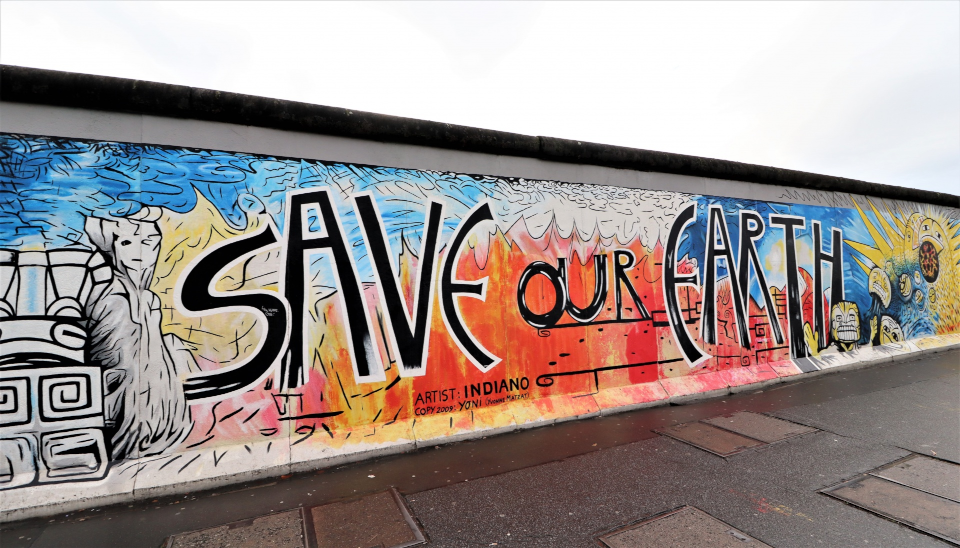
\includegraphics[scale=\myscale,scale=0.9]{figures/image-mur-avant}
	\end{minipage}\qquad
	\begin{minipage}{0.5\textwidth}
		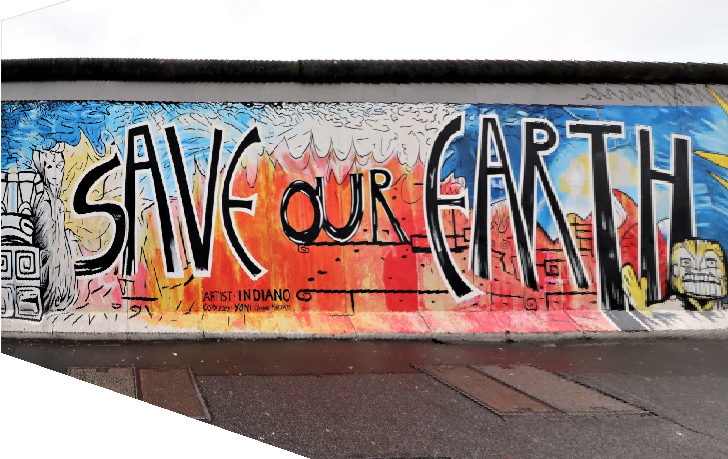
\includegraphics[scale=\myscale,scale=0.3]{figures/image-mur-apres}    
	\end{minipage}
\end{center}

Voici les équations de $\psi = \varphi^{-1} : (x,y) \mapsto (u,v)$ :
$$
u = \frac{-a_0b_2 + a_2 b_0 + (- b_0 c_2 + b_2) x + (a_0 c_2 - a_2) y }
{a_1 b_2 - a_2 b_1 + (b_1 c_2  - b_2 c_1) x + (- a_1 c_2  + a_2 c_1) y}
$$
et
$$
v = -\frac{-a_0 b_1 + a_1 b_0 + (- b_0 c_1  + b_1) x + (a_0 c_1  - a_1) y}
{a_1 b_2 - a_2 b_1 + (b_1 c_2 - b_2 c_1) x + (-a_1 c_2 + a_2 c_1) y}.
$$

%--------------------------------------------------------------------
\subsection{Cube}

Pour texturer un cube, on se donne souvent l'image du patron regroupant les $6$ faces dépliées.

\myfigure{1.1}{
	\tikzinput{fig-cube-01} \qquad\qquad 
	\tikzinput{fig-cube-03}
}

%--------------------------------------------------------------------
\subsection{Cylindre}

Pour appliquer une texture sur un cylindre ou une portion de ce cylindre on utilise bien sûr les coordonnées cylindriques (voir le chapitre \og{}Trigonométrie\fg{}).
Par exemple pour appliquer une texture de $[0,1]^2$ vers un cylindre de rayon $r$ et de hauteur $h$, on applique la fonction :
$$\Phi : (u,v)  \longmapsto (r, \theta, z) = (r, 2\pi u, hv)$$
où $(r,\theta,z)$ sont les coordonnées cylindriques.

\begin{center}
    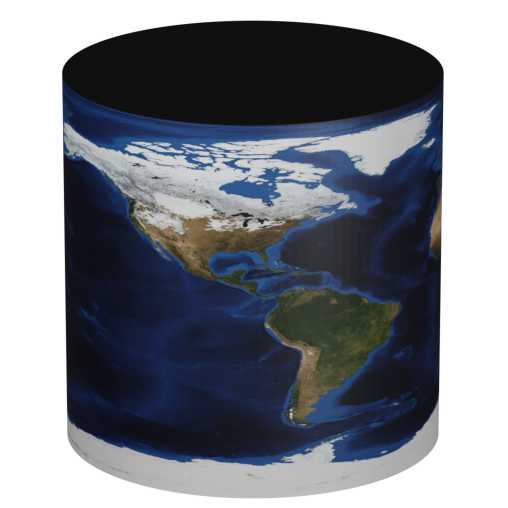
\includegraphics[scale=\myscale,scale=0.30]{figures/cylindre-texture}    
\end{center}

Si on souhaite n'appliquer la texture que sur une petite partie du cylindre (par exemple une petite étiquette sur un bouteille) et si cette partie est délimitée en coordonnées cylindriques par $\theta_1 \le \theta \le \theta_2$ et $z_1 \le z \le z_2$ alors l'application de texture serait :
$$\Phi : (u,v)  \longmapsto (r, \theta, z) = \big(r, (1-u)\theta_1+u\theta_1 , (1-v)z_1+vz_2 \big).$$
 
 
%--------------------------------------------------------------------
\subsection{Sphère}

Pour appliquer une texture sur une sphère de rayon $r$ on utilise les coordonnées sphériques $(r,\varphi,\lambda)$ (où $\varphi \in [-\frac\pi2,\frac\pi2]$ est la latitude et $\lambda\in [-\pi,\pi]$)  est la longitude) :
$$\Phi : (u,v)  \longmapsto (r,\varphi,\lambda) = \left(r, \pi(v-\tfrac12), 2\pi(v-\tfrac12)\right).$$
Le centre $(\frac12,\frac12)$ de la texture est envoyé sur le point de la sphère de latitude et longitude nulle.

\begin{center}
	\begin{minipage}{0.45\textwidth}
    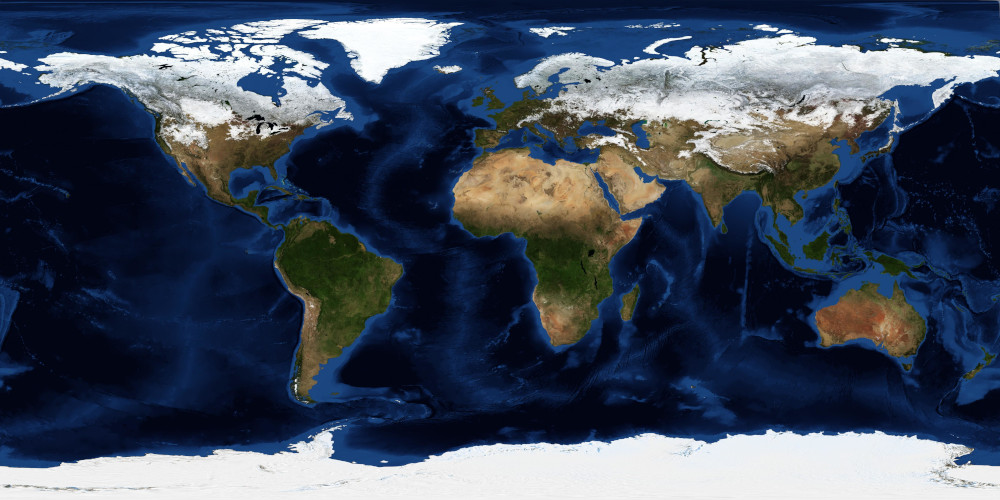
\includegraphics[scale=\myscale,scale=0.8]{figures/carte-monde-nasa}
    \end{minipage}\qquad 
	\begin{minipage}{0.5\textwidth}
    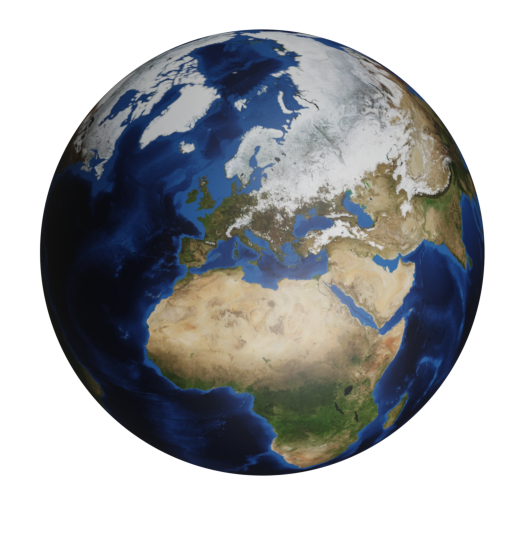
\includegraphics[scale=\myscale,scale=0.35,trim={0 2cm 0 1cm},clip]{figures/sphere-texture}    
    \end{minipage}
\end{center}


%--------------------------------------------------------------------
\subsection{Du cube vers la sphère}

Nous avons vu qu'il est très facile de réaliser le texturage d'un cube à l'aide de son patron.
Pour texturer une sphère il peut être intéressant de d'abord texturer un cube puis de le déformer en une sphère. Comme les équations générales peuvent devenir assez compliquées on va s'intéresser au problème du plan : comment transformer un carré vers un cercle (et inversement) ?

Considérons le carré $C = [-1,1]^2$ (de côté de longueur $2$) et le disque (fermé) $D$ de centre $(0,0)$ et de rayon $1$.
On note $(x,y)$ avec $-1 \le x \le 1$ et $-1 \le y \le 1$ les coordonnées pour le carré et $(u,v)$ avec $u^2+v^2 \le 1$ les coordonnées pour le disque. Il y a plusieurs façons de déformer un disque en un carré

\myfigure{1.2}{
	\tikzinput{fig-carre-cercle-01}
}


\textbf{Méthode 1 : rayons.}
Le disque $D$ est inclus dans le carré $C$. Pour un point $P$ du bord du disque $D$, on trace le rayon issu de l'origine, ce rayon recoupe le bord du carré $C$ en $Q$ qui sera l'image de $P$. 
Si maintenant $P$ est un point intérieur à $D$, il est situé sur un cercle de rayon $r$ centré à l'origine, on effectue le même procédé pour envoyer ce point sur le carré de côté $2r$. Ainsi chaque cercle concentrique est envoyé sur un carré.

\myfigure{1}{
	\tikzinput{fig-carre-cercle-02}
}

Les équations $F : D \to C$, $(u,v) \mapsto (x,y)$ pour passer d'un disque à un carré sont données par :
$$x = \begin{cases}
	\sgn(u) \sqrt{u^2+v^2} & \text{ si } u^2 \ge v^2 \\
	\sgn(v) \frac uv \sqrt{u^2+v^2} & \text{ si } u^2 < v^2 \\
\end{cases}
\qquad\qquad
y = \begin{cases}
	\sgn(u)\frac vu \sqrt{u^2+v^2} & \text{ si } u^2 \ge v^2 \\
	\sgn(v)\sqrt{u^2+v^2} & \text{ si } u^2 < v^2 \\
\end{cases}
$$
La fonction signe, notée $\sgn(x)$, est définie par :
$$\sgn(x) = \begin{cases}
	+1 & \text{ si } x > 0 \\
	0  &  \text{ si } x = 0 \\
	-1 & \text{ si } x < 0 \\
\end{cases}$$
Pour $x \neq 0$ on a aussi $\sgn(x) = \frac{x}{|x|}$.

Voici le disque et sa transformation en un carré :
\begin{center}
	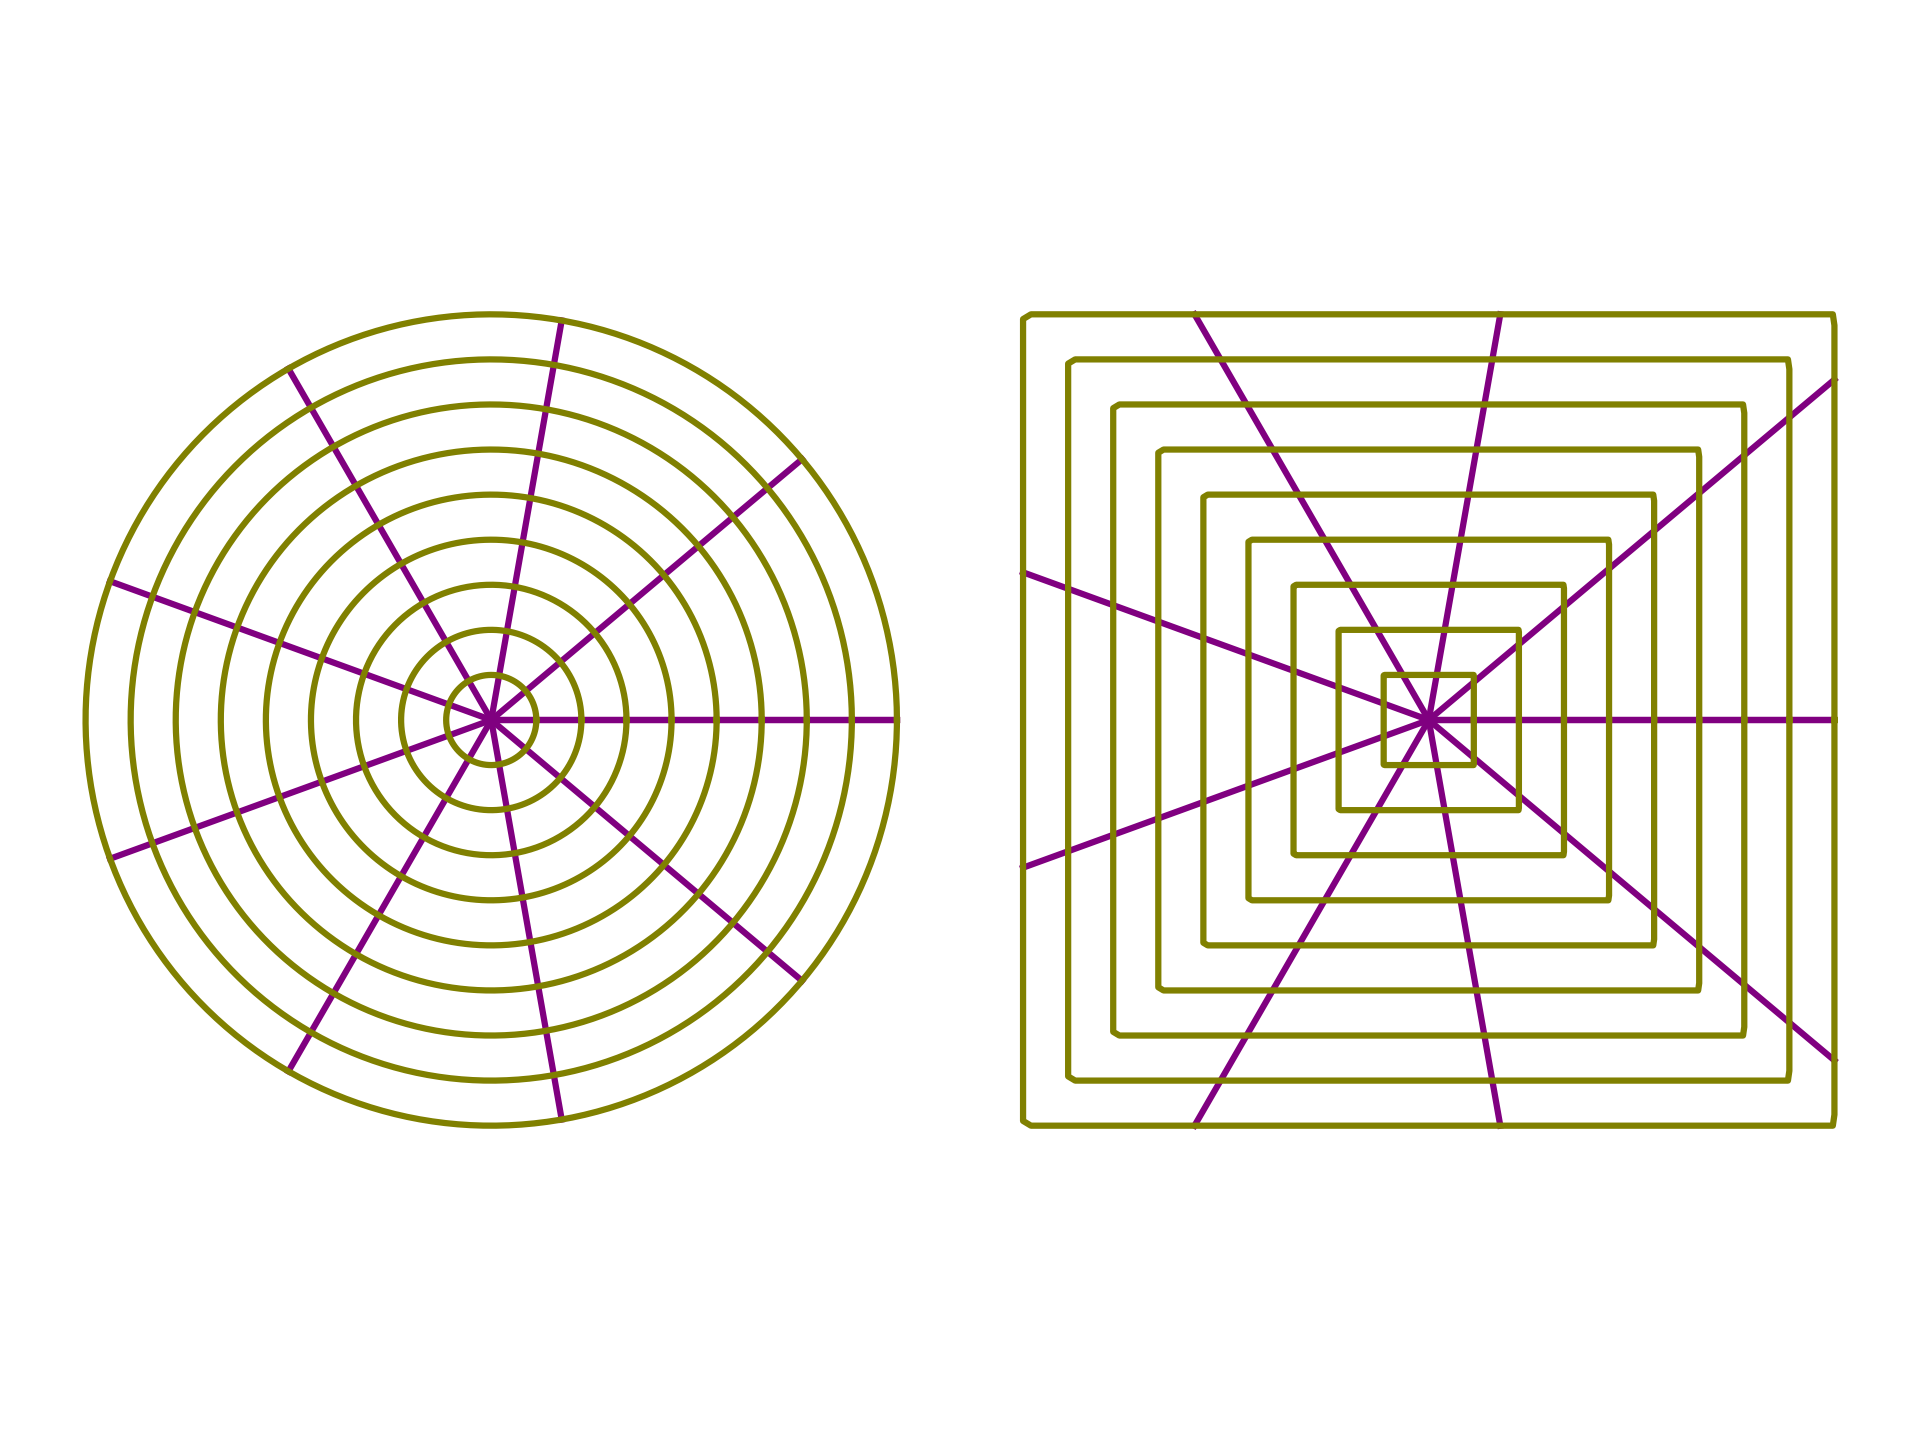
\includegraphics[scale=\myscale,scale=0.5,trim={0 2cm 0 2cm},clip]{figures/carre-cercle-02}
\end{center}


Les équations inverses $G : C \to D$, $(x,y) \mapsto (u,v)$ permettent de passer du carré au disque :
$$u = \begin{cases}
	\sgn(x) \frac{x^2}{\sqrt{x^2+y^2}} & \text{ si } x^2 \ge y^2 \\
	\sgn(y) \frac{xy}{\sqrt{x^2+y^2}} & \text{ si } x^2 < y^2 \\
\end{cases}
\qquad\qquad
v = \begin{cases}
	\sgn(x) \frac{xy}{\sqrt{x^2+y^2}} & \text{ si } x^2 \ge y^2 \\
	\sgn(y) \frac{y^2}{\sqrt{x^2+y^2}} & \text{ si } x^2 < y^2 \\
\end{cases}
$$

Voici le carré et sa transformation en un disque :
\begin{center}
	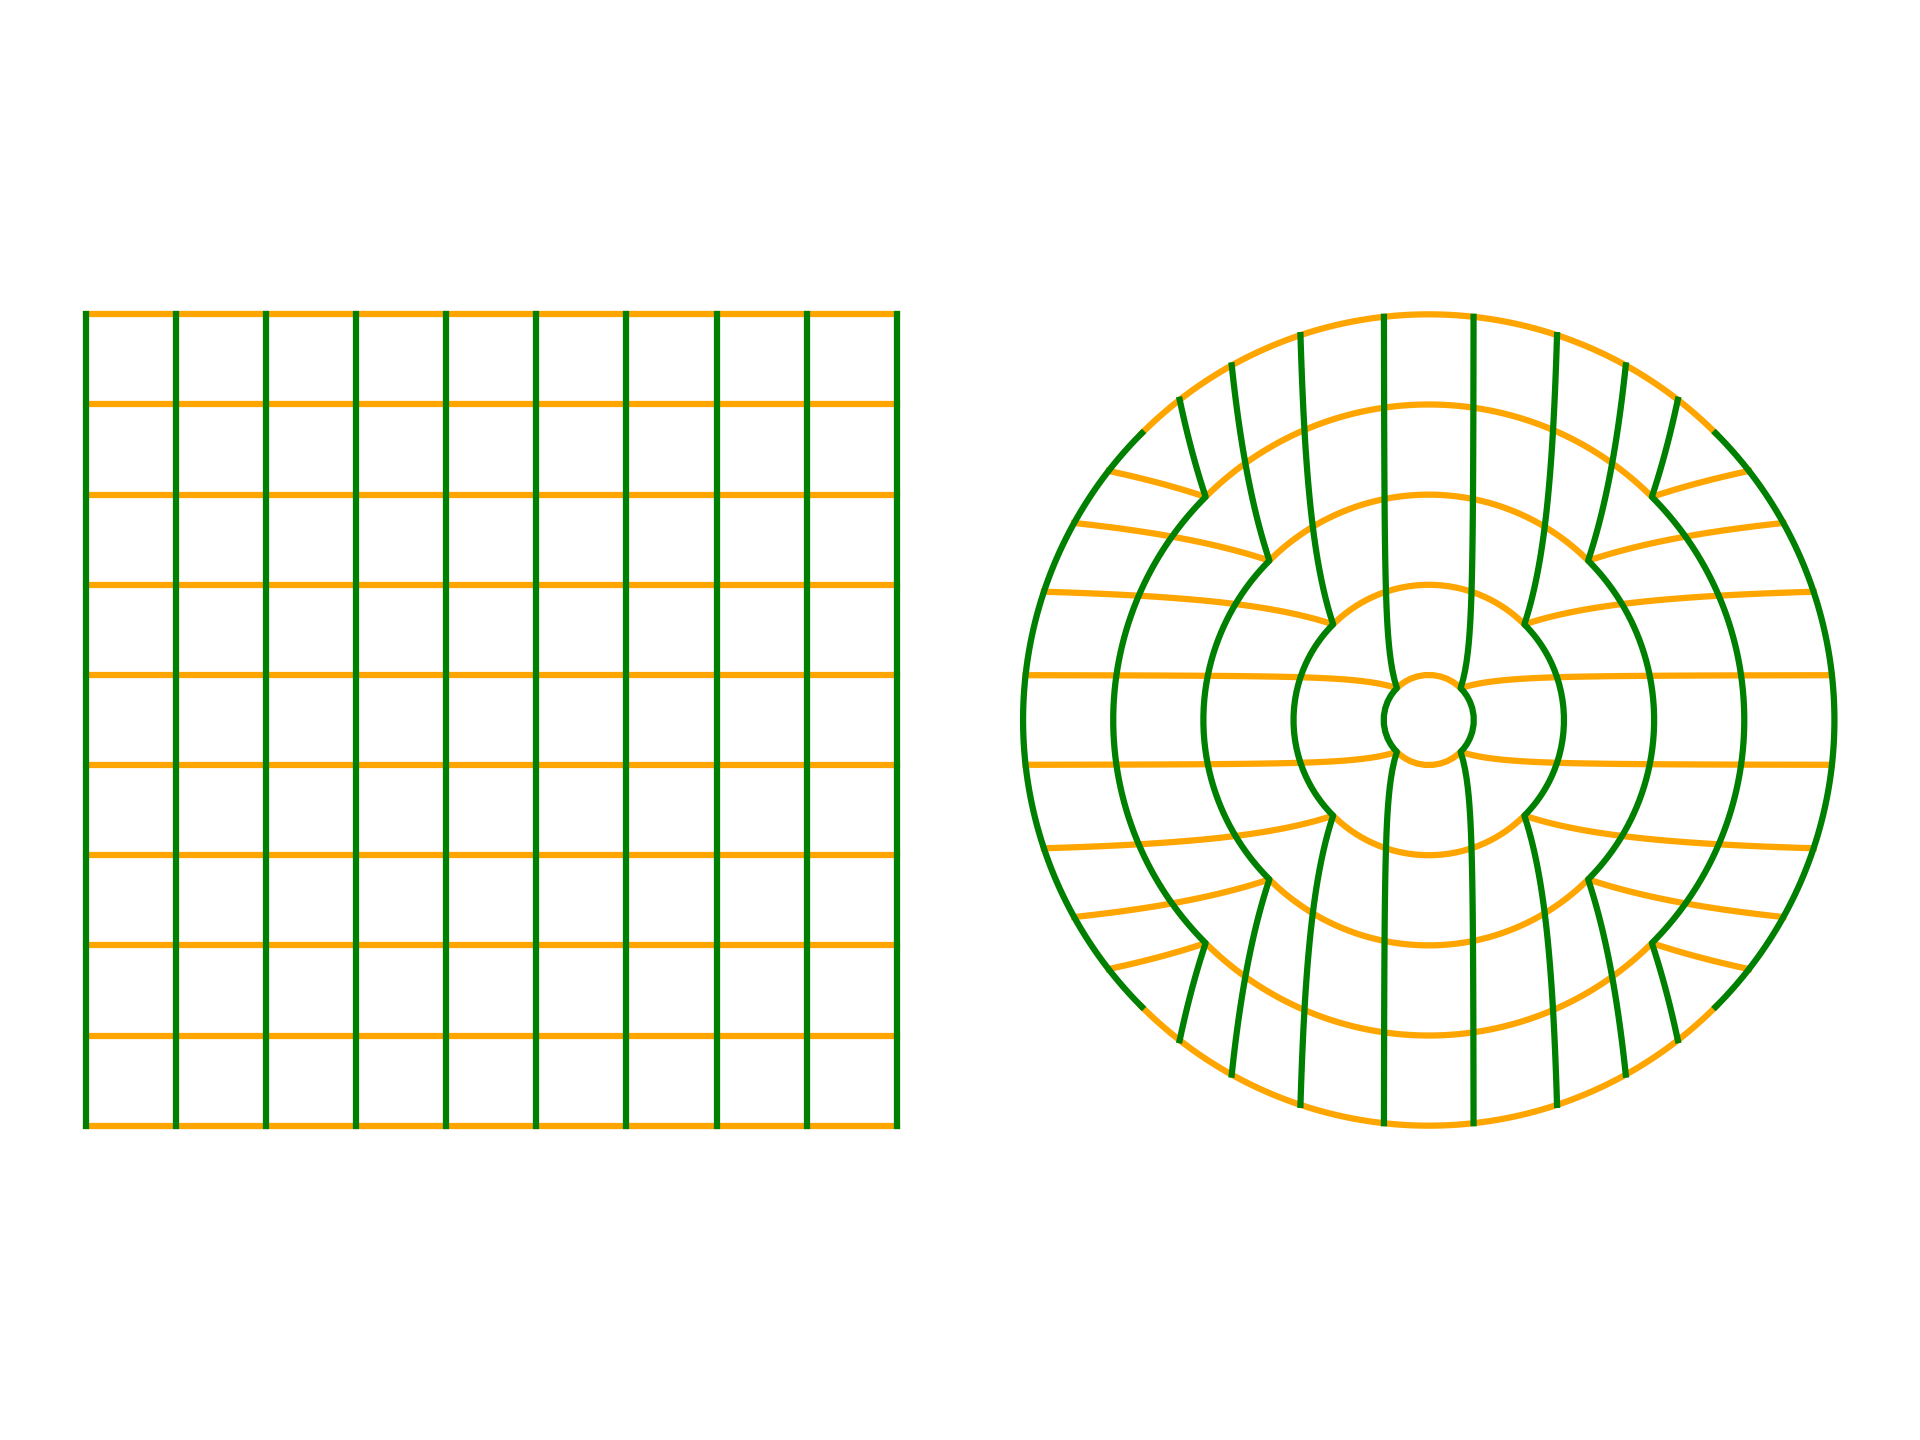
\includegraphics[scale=\myscale,scale=0.5,trim={0 2cm 0 2cm},clip]{figures/carre-cercle-01}
\end{center}

\medskip

\textbf{Méthode 2 : via des ellipses.}
Voyons une méthode un peu plus régulière pour déformer un disque en un carré. 
Un segment vertical du carré est envoyé sur une portion d'ellipse dans le disque, de même pour des segment horizontaux.
Les équations $G : C \to D$, $(x,y) \mapsto (u,v)$ qui permettent de passer du carré au disque sont particulièrement simples :
$$u = x \sqrt{1-\frac{y^2}{2}}
\qquad\qquad
v = y \sqrt{1-\frac{x^2}{2}}
$$

Les équations $F : D \to C$, $(u,v) \mapsto (x,y)$ pour passer d'un disque à un carré sont données par :
\begin{align*}
x &= 
	\frac12 \sqrt{2 + u^2 - v^2 +2 \sqrt{2}u}
	- \frac12 \sqrt{2 + u^2 - v^2 - 2\sqrt{2}u} \\
y &= \frac12 \sqrt{2 - u^2 + v^2 + 2 \sqrt{2}v}
- \frac12 \sqrt{2 - u^2 + v^2 - 2\sqrt{2}v}
\end{align*}


Voici le carré et sa transformation en un disque : 
\begin{center}
	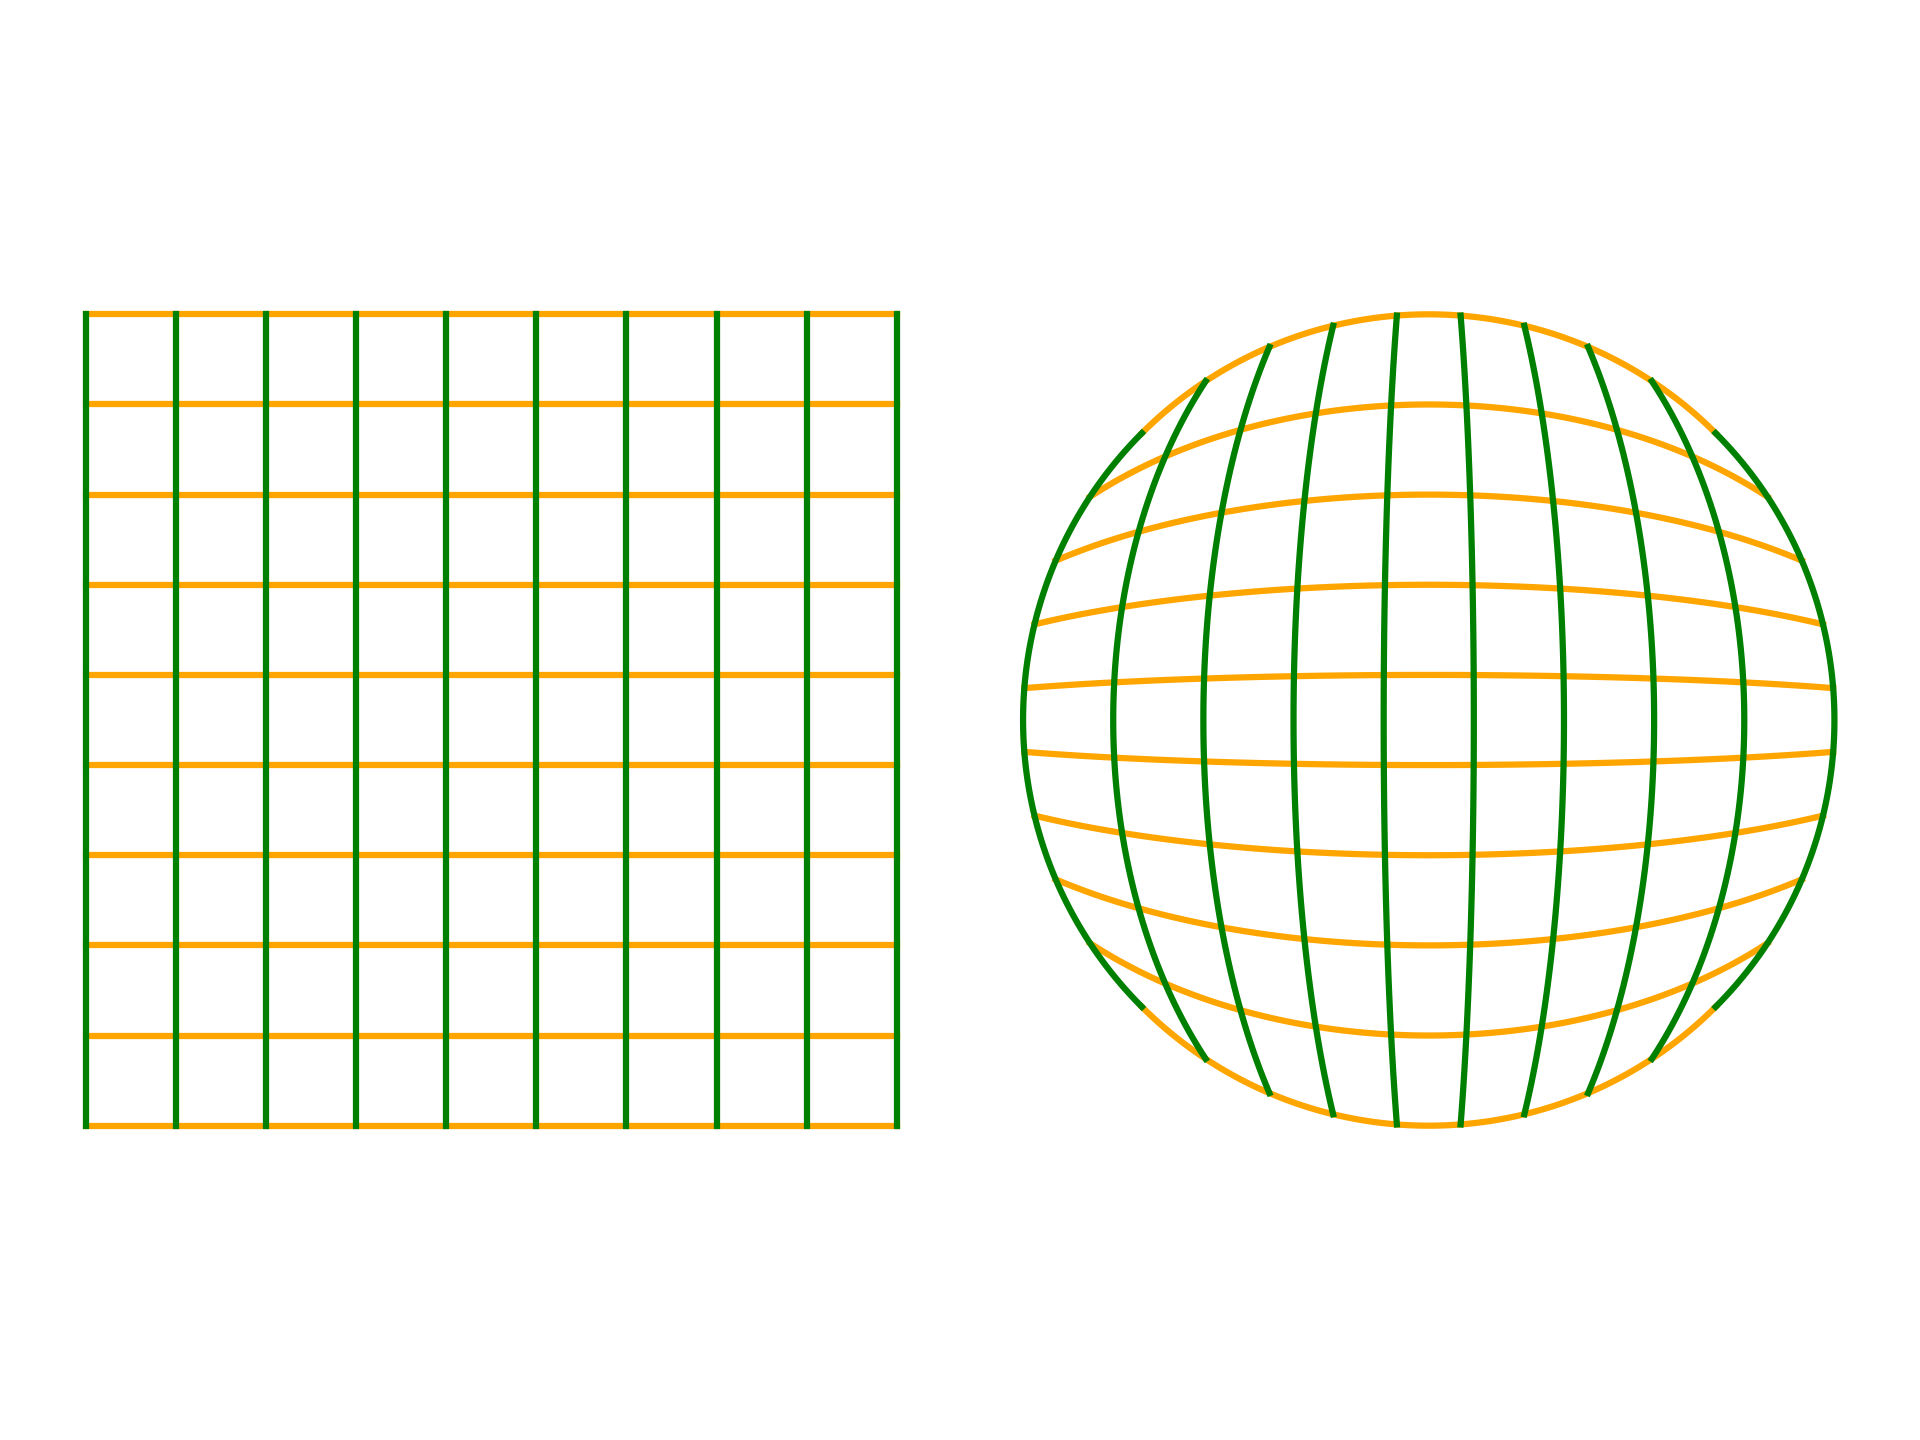
\includegraphics[scale=\myscale,scale=0.5,trim={0 2cm 0 2cm},clip]{figures/carre-cercle-03}
\end{center}

Voici le disque et sa transformation en un carré :
\begin{center}
	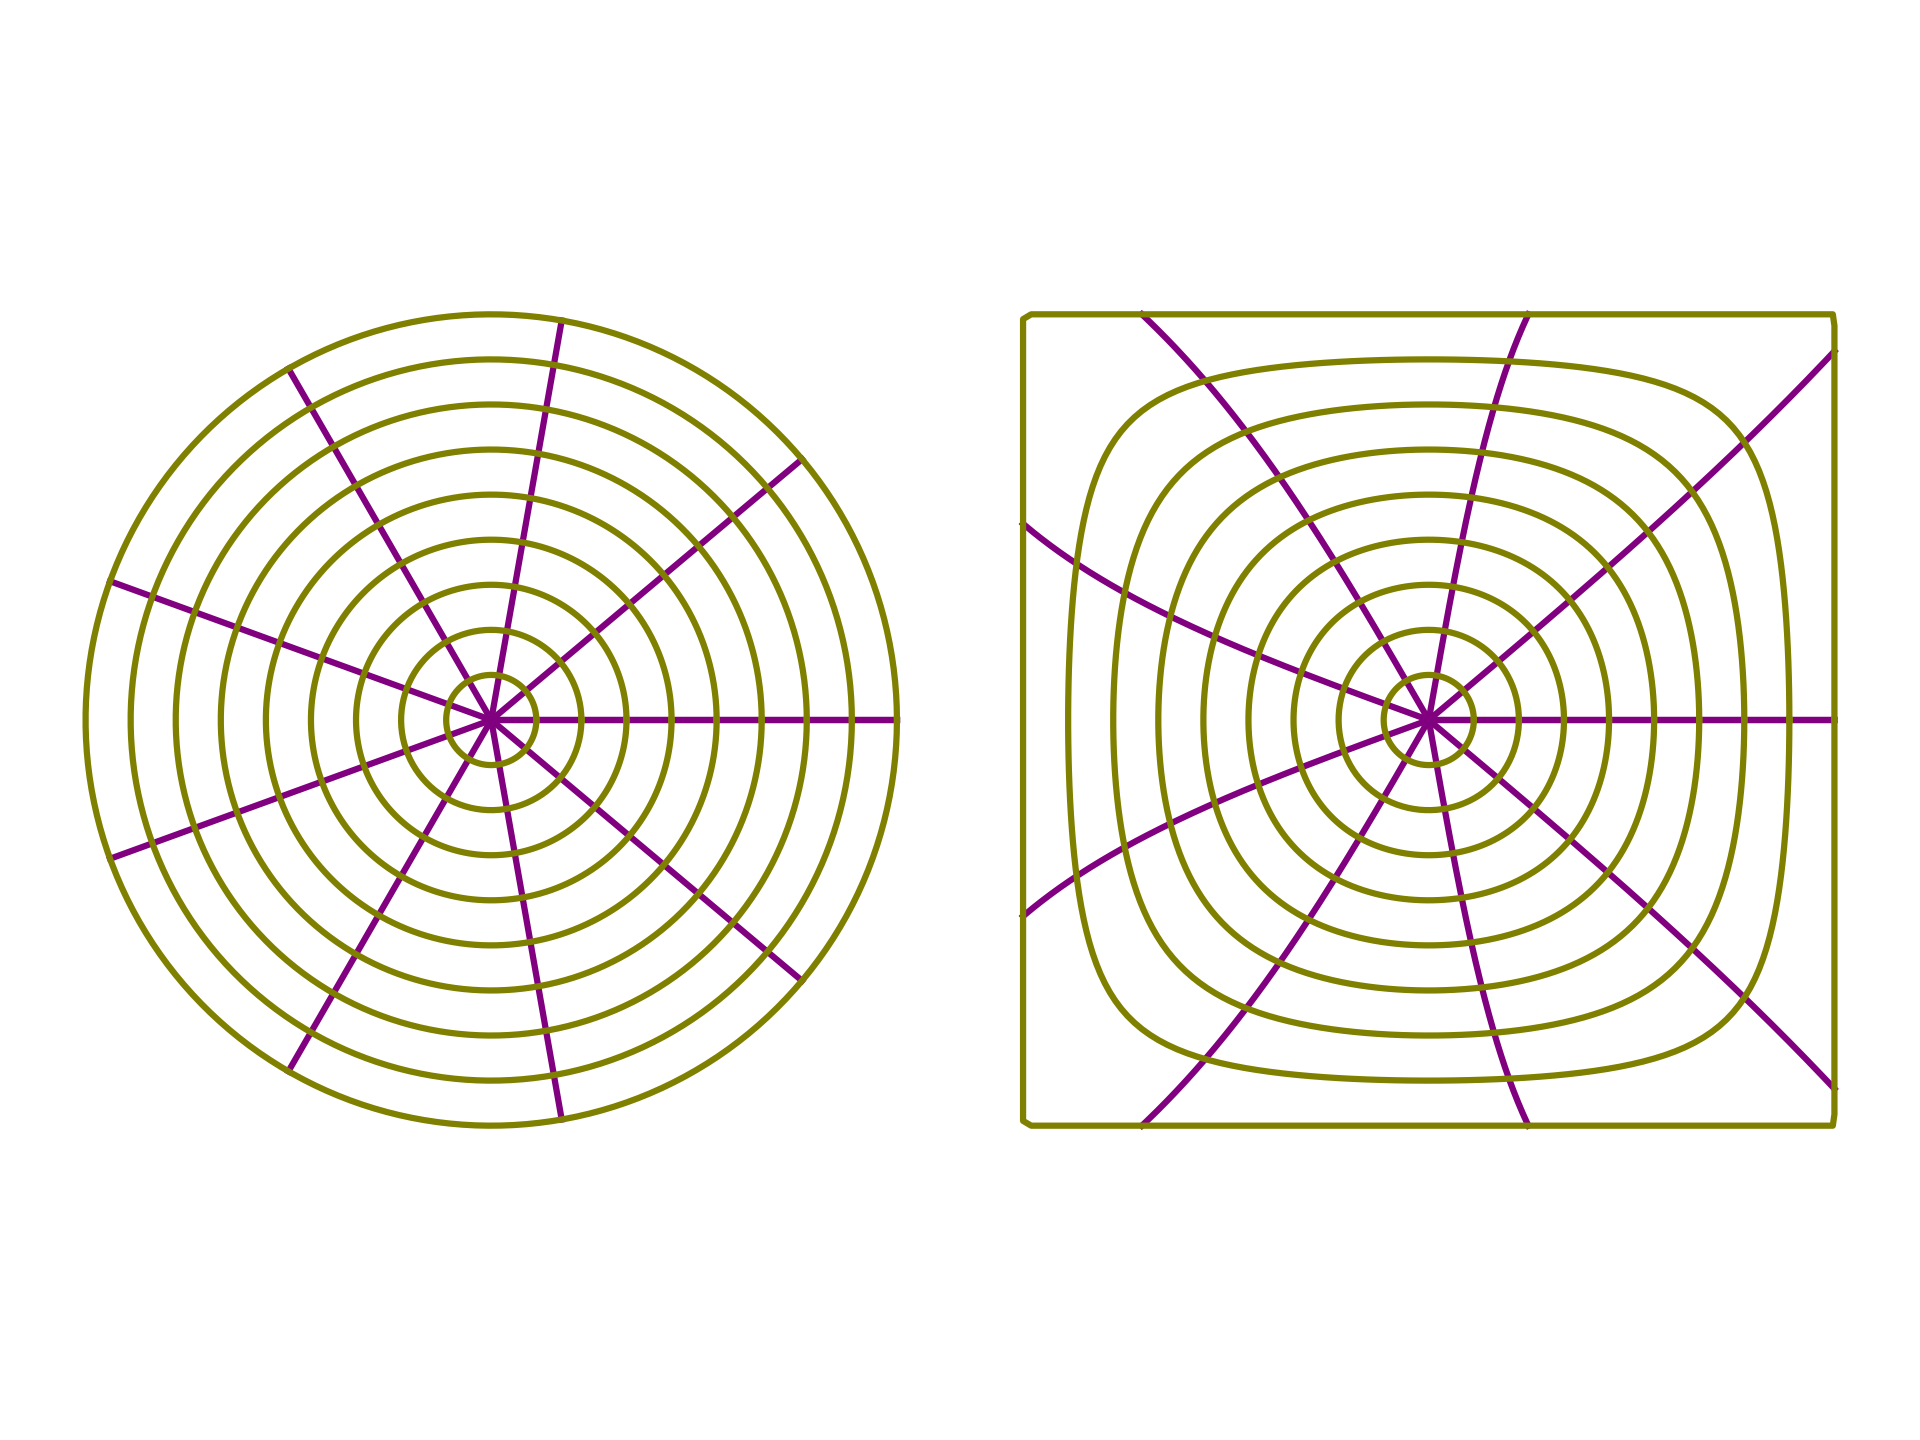
\includegraphics[scale=\myscale,scale=0.5,trim={0 2cm 0 2cm},clip]{figures/carre-cercle-04}
\end{center}

On transforme ainsi facilement une image carrée en une image ronde (à gauche l'image originale, au centre la méthode 1, à droite la méthode 2) :
\begin{center}
	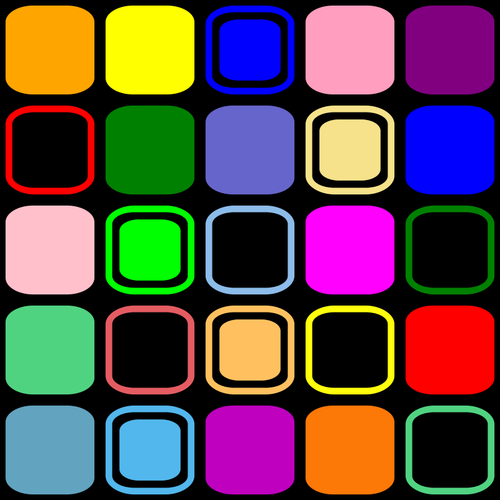
\includegraphics[scale=\myscale,scale=0.23]{figures/image_carre_avant} \qquad
	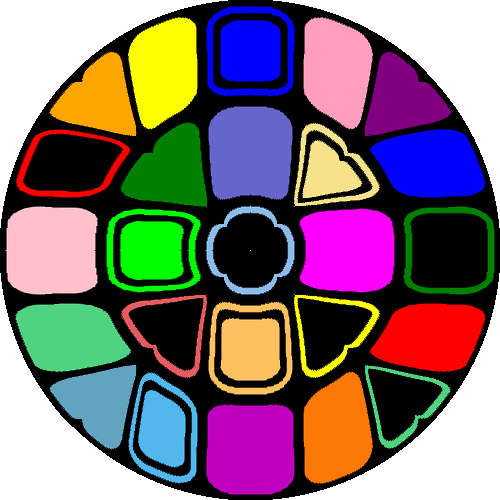
\includegraphics[scale=\myscale,scale=0.25]{figures/image_carre_apres_1} \qquad	
	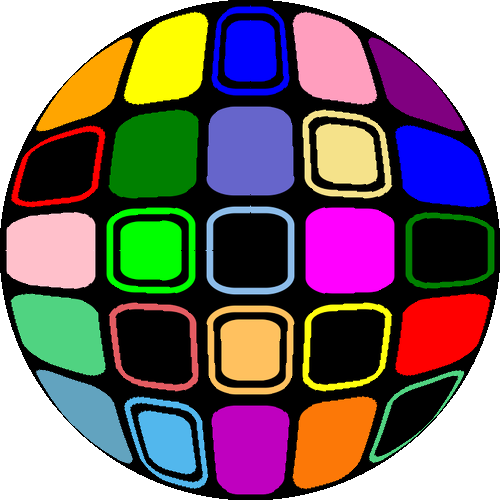
\includegraphics[scale=\myscale,scale=0.25]{figures/image_carre_apres_2}		
\end{center}

Et une image ronde vers une image carrée  (à gauche l'image originale, au centre la méthode 1, à droite la méthode 2) :
\begin{center}
	
\includegraphics[scale=\myscale,scale=0.32]{figures/image_disque_avant} \qquad
	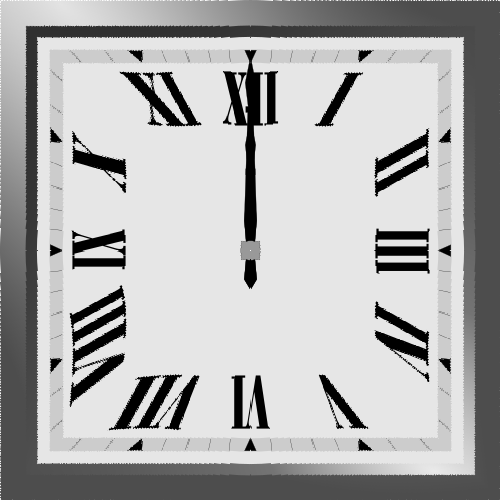
\includegraphics[scale=\myscale,scale=0.25]{figures/image_disque_apres_1} \qquad	
	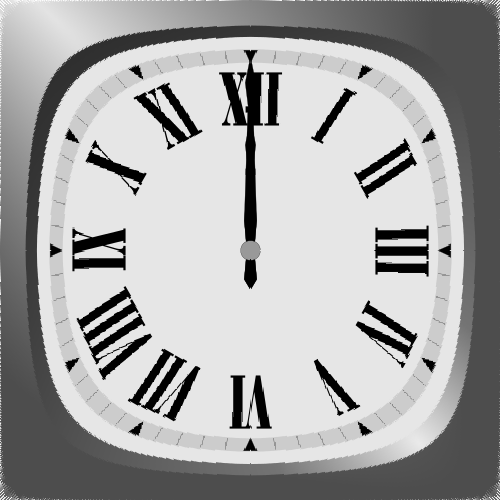
\includegraphics[scale=\myscale,scale=0.25]{figures/image_disque_apres_2}		
\end{center}


Ces équations  et beaucoup d'autres sont à retrouver dans  \href{https://arxiv.org/pdf/1509.06344.pdf}{\emph{Analytical methods for squaring the disc}} de Chamberlain Fong. 
	
\medskip

\textbf{Du cube vers la sphère.}
Voici les équations de la fonction $G : (x,y,z) \mapsto (u,v,w)$, analogue à la version elliptique ci-dessus, qui permettent de passer du cube $[-1,1]^3$ (avec les coordonnées $(x,y,z)$) à la boule de rayon $1$ centrée à l'origine (définie par $u^2+v^2+w^2 \le 1$).
\begin{align*}
u  &= x\sqrt{1-\frac{y^2}{2}-\frac{z^2}{2}+\frac{y^2z^2}{3}} \\
v  &= y\sqrt{1-\frac{x^2}{2}-\frac{z^2}{2}+\frac{x^2z^2}{3}} \\
w  &= z\sqrt{1-\frac{x^2}{2}-\frac{y^2}{2}+\frac{x^2y^2}{3}} \\
\end{align*}




\end{document}




%\myfigure{0.7}{
	%    \tikzinput{texture-01}
	%}
%
%\begin{center}
%    \includegraphics[scale=\myscale,scale=0.5]{figures/texture-01}
%\end{center}